%%
%
% ARQUIVO: main.tex
%
% VERSÃO: 1.0
% DATA: Maio de 2016
% AUTOR: Coordenação de Trabalhos Especiais SE/8
% 
%  Arquivo tex principal do documento de Projeto de Fim de Curso (PFC).
%  Este arquivo SÓ PRECISA SER MODIFICADO NA PARTE DE CONTEÚDO:
%
%    a. colocar um \include{•} para cada capítulo do documento de PFC.
%
%%

% -----
% CLASSE DO DOCUMENTO DE PFC
% -----
\documentclass{pfc}

% -----
% PACOTES LATEX USADOS NO DOCUMENTO DE PFC
% -----
\usepackage[brazilian]{babel}
\usepackage[utf8]{inputenc}
\usepackage[T1]{fontenc}

\usepackage{graphicx}
\usepackage{tabularx}
\usepackage{float}
\usepackage{color}
\usepackage{amsfonts,amssymb}
\usepackage[authoryear]{natbib}

\usepackage{enumitem}
\usepackage{rotating}
\usepackage{lipsum}
\usepackage{lastpage}
\usepackage{stringstrings}
\usepackage{pgffor}
\usepackage{pdftexcmds}
\usepackage{algorithm2e}
\usepackage{amsmath}

% -----
% MARGENS DO DOCUMENTO DE PFC
% -----
\usepackage{geometry}
\geometry{
	a4paper,
	total={210mm,297mm},
	left=25mm,
	right=25mm,
	top=25mm,
	bottom=30mm,
	textwidth=160mm,
	textheight=242mm,
	headheight=0mm,
	headsep=0mm,
}

% -----
% DECLARAÇÕES AUXILIARES PARA REFERÊNCIAS
%
%  Diferencia \citet e \citep de acordo com a NBR 10520:2002
% -----
\DeclareRobustCommand{\NATand}{;}
\DeclareRobustCommand{\NATetal}{et~al.}
\makeatletter
\renewcommand{\NAT@nmfmt}[1]{%
  \ifNAT@swa\expandafter\MakeUppercase
  \else\DeclareRobustCommand{\NATand}{ e}\expandafter\@firstofone\fi{{\NAT@up #1}}%
}
\makeatother

% -----
% AMBIENTE DE FIGURAS DE PFC
%
%  A classe do documento está configurada SOMENTE para figuras no formato EPS.
%  Logo, use PREFERENCIALMENTE este tipo de arquivo.
%
%    a. os arquivos das figuras devem estar no diretório 'img'
% -----
\graphicspath{{./img/}}

% -----
% INÍCIO DO DOCUMENTO DE PFC
% -----
\begin{document}

% -----
% PARTE PRÉ-TEXTUAL DE PFC
%
% Alterar o CONTEÚDO dos arquivos siglas.tex E pre-texto.tex
% -----
%%
%
% ARQUIVO: dados-pfc.tex
%
% VERSÃO: 1.0
% DATA: Maio de 2016
% AUTOR: Coordenação de Trabalhos Especiais SE/8
% 
%  Arquivo tex com os dados acerca do documento de PFC e da apresentação.
%
%   nos campos que definem nomes (autor; orientador; co-orientador; membros da banca)
%   É PRECISO usar os COMANDOS LaTeX para acentuação, conforme abaixo:
%
%         \'a - á || \`a - à || \~a - ã || \^a - â 
%         \'e - é || \^e - ê || \'i - í 
%         \'o - ó || \~o - õ || \^o - ô 
%         \'u - ú || \"u - ü
%
%%

%%% AUTORES DO PFC (Nome completo)
% ---
%  aceita até 03 autores (de autorI até autorIII)
%    a. preencher sucessivamente a partir de autorI
%    b. REMOVER as definições não necessárias
% ---
\autorI{Bruno Avelino de Araujo Oliveira}
\autorII{Jayme Boarin de Magalhães Alvim}

%%% POSTOS DOS AUTORES DO PFC
% ---
%  aceita os postos de até 03 autores (de postoautorI até postoautorIII)
%    a. preencher sucessivamente a partir de postoautorI (que deve ser o posto de autorI)
%    b. se o autorX É CIVIL, NÃO DEFINIR postoautorX (remover a linha de definição)
%    c. se o autorX É MILITAR, DEFINIR postoautorX com UMA das seguintes ALTERNATIVAS: Alu / 1 Ten / Cap
% ---
\postoautorI{Cap}

%%% TITULO DO PFC
\titulo{Desenvolvimento de Algoritmos de Segmentação de Imagens em Ambiente Android}

%%% DATA DA APRESENTAÇÃO (formato {dd}{Mmmmm}{aaaa})
\datadefesa{18}{Maio}{2017}

%%% ORIENTADOR DO PFC
% ---
%  CAMPO 1: P (para Prof.); PA (para Profa.); ou qualquer coisa (inclusive VAZIO) - o que for escrito aparecerá no documento
%  CAMPO 2: Nome completo
%  CAMPO 3: D (para D.Sc.); P (para Ph.D.); M (para M.Sc.) ou qualquer coisa (inclusive VAZIO) - o que for escrito aparecerá no documento
%  CAMPO 4: Instituição (com "do / da")
% ---
\orientador{PA}{Carla Liberal Pagliari}{P}{do IME}

%%% CO-ORIENTADOR DO PFC
% ---
%  se não houver co-orientador, REMOVA ESTA LINHA
%  preenchimento idêntico a \orientador{}{}{}{}
% ---
\coorientador{P}{Marcelo de Mello Perez}{P}{do IME}

%%% NÚMERO DA ENTRADA DA BIBLIOTECA (pegar na Biblioteca do IME)
% \biblioref{004.69}{S586e}

%%% PALAVRAS-CHAVES DO PFC
% ---
%  devem ser separadas por vírgula e É OBRIGATÓRIO ter pelo menos uma
% ---
\palavraschaves{Segmentação, Imagem, Visão Computacional, Algoritmos}

%%% OUTROS MEMBROS DA BANCA DO PFC
% ---
%  aceita até mais 05 membros (de membrobancaI até membrobancaV)
%    a. preencher sucessivamente a partir de membrobancaI
%    b. REMOVER as definições não necessárias
%
%  cada membro tem preenchimento idêntico a \orientador{}{}{}{}
% ---
\membrobancaI{P}{Anderson Fernandes Pereira dos Santos}{D}{do IME}
\membrobancaII{P}{Paulo Roberto Rosa Lopes Nunes}{P}{do IME}
%\membrobancaIII{}{Nome do Membro da Banca 3}{}{da COPPE/UFRJ}
%\membrobancaIV{}{Nome do Membro da Banca 4}{}{da UNIRIO}
%\membrobancaV{}{Nome do Membro da Banca 5}{}{da UERJ}


%%
%
% ARQUIVO: pre-texto.tex
%
% VERSÃO: 1.0
% DATA: Maio de 2016
% AUTOR: Coordenação de Trabalhos Especiais SE/8
% 
%  Arquivo tex para a criação da parte pré-textual do documento de Projeto de Fim de Curso.
%
%%


% -----
% PÁGINA DE CAPA DO DOCUMENTO DE PFC
% -----
\makecapa

% -----
% PÁGINA DE TÍTULO DO PFC
% -----
\prepareadvisors
\maketitle

% -----
% PÁGINA DE CRÉDITOS DO DOCUMENTO DE PFC
% -----
\makecredits

% -----
% PÁGINA DE FOLHA DE ASSINATURAS
% -----
\preparemembers
\approvalpage

% -----
% PÁGINA DE DEDICATÓRIA (OPCIONAL, ie. pode remover toda a página)
% -----
%%% DEDICATÓRIA - PREENCHER...
% -----
% PÁGINA DE DEDICATÓRIA (OPCIONAL, ie. pode remover toda a página)
% -----
%%% DEDICATÓRIA - PREENCHER...
\dedicatoria{%
Dedico aos meus familiares, amigos, minha esposa Mayra e professores do Instituto Militar de Engenharia, pois me deram forças e foram fundamentais para que eu pudesse vencer os obstáculos diários. 
Dedico aos meus pais e familiares pelo amor incondicional e pelos valores e ensinamentos passados que me fazem crescer e evoluir constantemente.
}%
\makededication

% -----
% PÁGINA DE AGRADECIMENTOS (OPCIONAL, ie. pode remover toda a página)
% -----
%%% AGRADECIMENTOS - PREENCHER...
\agradecimentos{%
Agradeço aos que estiveram comigo durante essa árdua jornada de estudos e me auxiliaram nessa etapa de desenvolvimento profissional. 
Um muito obrigado aos familiares, amigos e mestres.\\
\indent
Um obrigado especial aos Professores Orientadores Ph.D. Carla Liberal Pagliari e Ph.D. Marcelo de Mello Perez, por suas disponibilidades e atenções.
}%
\makethanks

% -----
% PÁGINA DE EPÍGRAFE (OPCIONAL, ie. pode remover toda a página)
% -----
%%% EPÍGRAFE - PREENCHER...
\epigrafe{%
“Computação não se relaciona mais a computadores. Relaciona-se a viver.”%
}%
\autorepigrafe{%    %% Se não tem autor, coloque "Anônimo"
Nicholas Negroponte%
}%
\makeepigraph

% -----
% PÁGINA DE SUMÁRIO
% -----
\tableofcontents

% -----
% PÁGINAS DE LISTAS DE FIGURAS E DE TABELAS
% se a Dissertação não possui figuras e/ou tabelas, REMOVA O COMANDO CORRESPONDENTE
% -----
\listoffigures
\listoftables

% -----
% PÁGINA DE LISTA DE SIGLAS
% se a Dissertação não possui siglas, REMOVA TODA A PÁGINA
% -----
%%% SIGLAS - PREENCHER...
% \acronimo{LA}{Los Angeles}


 \listofnicks

% -----
% PÁGINA DE LISTA DE ABREVIATURAS
% se a Dissertação não possui abreviaturas ou símbolos, REMOVA TODA A PÁGINA
% -----
%%% ABREVIATURAS - PREENCHER...
\abreviatura{T}{Threshold}
\abreviatura{fij}{píxel na posição (i,j) }

%%% SÍMBOLOS - PREENCHER...
\simbolo{$\Phi$}{termo de dissipação visco	sa}
\simbolo{$\Gamma$}{coeficiente de difusão efetivo}
\simbolo{$\alpha$}{fator de sub-relaxação}
\simbolo{$\phi$}{variável dependente da equação diferencial geral}

% \listofsymbols

% -----
% PÁGINA DE RESUMO
% -----
%%% RESUMO - PREENCHER...
\resumo{%
At vero eos et accusamus et iusto odio dignissimos ducimus qui blanditiis praesentium voluptatum deleniti atque corrupti quos dolores et quas molestias excepturi sint occaecati cupiditate non provident, similique sunt in culpa qui officia deserunt mollitia animi, id est laborum et dolorum fuga. Et harum quidem rerum facilis est et expedita distinctio. Nam libero tempore, cum soluta nobis est eligendi optio cumque nihil impedit quo minus id quod maxime placeat facere possimus, omnis voluptas assumenda est, omnis dolor repellendus.\\
\indent
Temporibus autem quibusdam et aut officiis debitis aut rerum necessitatibus saepe eveniet ut et voluptates repudiandae sint et molestiae non recusandae. Itaque earum rerum hic tenetur a sapiente delectus, ut aut reiciendis voluptatibus maiores alias consequatur aut perferendis doloribus asperiores repellat.
}%
% \makeresumo

% -----
% PÁGINA DE ABSTRACT
% -----
%%% ABSTRACT - PREENCHER...
\abstract{%
\lipsum[1]
}%
% \makeabstract


\parindent 0.75cm

% -----
% PARTE DE CONTEÚDO DE PFC
%
%  Escrever cada capitulo do documento de PFC em um arquivo .tex separado.
%  Adicionar os arquivos .tex ao documento com comando \include{•}
% -----
%%
%
% ARQUIVO: cap-01.tex
%
% VERSÃO: 1.0
% DATA: Maio de 2016
% AUTOR: Coordenação de Trabalhos Especiais SE/8
% 
%  Arquivo tex de exemplo de capítulo do documento de Projeto de Fim de Curso.
%
% ---
% DETALHES
%  a. todo capítulo deve começar com \chapter{•}
%  b. usar comando \noindent logo após \chapter{•}
%  c. citações para referências podem ser
%       i. \citet{•} para citações diretas (p. ex. 'Segundo Autor (2015)...'
%       ii. \citep{•} para citações indiretas (p. ex. '... (AUTOR, 2015)...'
%  d. notas de rodapé devem usar dois comandos
%       i. \footnotemark para indicar a marca da nota no texto
%       ii. \footnotetext{•}, na sequência, para indicar o texto da nota de rodapé
%  e. figuras devem seguir o exemplo
%       i. devem ficar no diretório /img e devem ser no formato EPS
%  f. tabelas devem seguir o exemplo
%  g. figuras e tabelas podem ser colocadas em orientação landscape
%       i. figuras: usar \begin{sidewaysfigure} ... \end{sidewaysfigure}
%                   em vez de \begin{figure} ... \end{figure}
%       ii. tabelas: usar \begin{sidewaystable} ... \end{sidewaystable}
%                    em vez de \begin{table} ... \end{table}
%  h. toda figura e tabela deve ser referenciada ao longo do texto com \ref{•}
% ---
%%

\chapter{Introdução}

\section{Motivação}
Cada vez mais as máquinas estão sendo utilizadas em atividades de nossa sociedade. Atuando na substituição de profissionais ou no auxílio dos mesmos, elas estão presentes e participando de nosso cotidiano ativamente. A implementação de sistemas de visão computacional tem se tornado, portanto, uma necessidade mais forte à medida que as aplicações que envolvem o tratamento de imagens se desenvolvem e buscam se aproximar da visão e da análise humana.
A segmentação é uma importante técnica utilizada nas atividades que envolvem o processamento digital de imagens. Diversas são as aplicações que fazem uso da identificação e análise de uma imagem, necessitando do estudo de regiões específicas das mesmas a fim de alcançar resultados e conclusões de forma eficiente.
Por se tratar de um problema sem solução universal e de vasta aplicação,  existem inúmeras possibilidades a serem exploradas e muito se tem estudado sobre essa área, com a evolução de novas técnicas e algoritmos que trazem uma nova abordagem ao problema.
%Esse projeto trará, portanto, um conhecimento mais profundo nesse importante domínio da Visão Computacional com a concepção de um produto que servirá tanto como base para estudo quanto uma base para futuros projetos mais avançados.
Esse projeto visa estudar e implementar técnicas de segmentação de imagens no ambiente Android, possibilitando o aprendizado de diferentes métodos da área de processamento de imagens, incluindo a área de visão computacional, bem como de desenvolvimento de aplicativos na plataforma Android. A Figura \ref{fig:tela_android} exibe o resultado do aplicativo que este projeto de final de curso está desenvolvendo.


% Figura -----------------------------------------------------------------------------------------------------------------------------
  \begin{figure}[!htb]
       \begin{center}  
          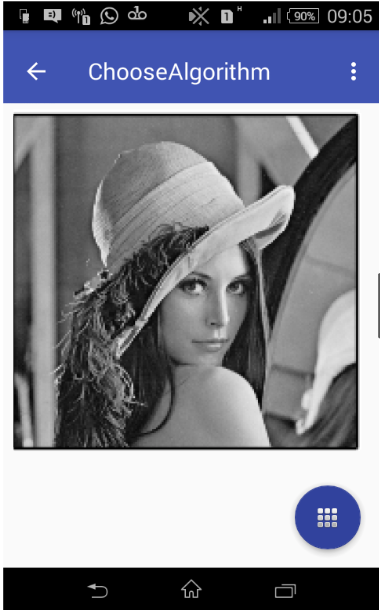
\includegraphics[width=0.2\columnwidth]{img/tela_android-original.png} \quad
          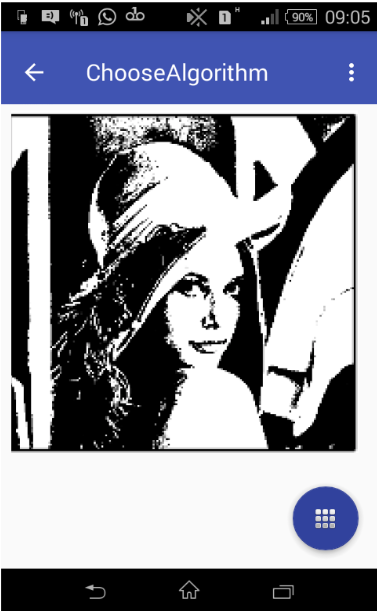
\includegraphics[width=0.2\columnwidth]{img/tela_android.png}
           \caption{\label{fig:tela_android}Tela do Aplicativo Android (imagem original e imagem segmentada).}
           % \vspace{2.0em}
       \end{center}
   \end{figure}
 % Figura -----------------------------------------------------------------------------------------------------------------------------

% um conhecimento mais profundo nesse importante domínio da Visão Computacional com a concepção de um produto que servirá tanto como base para estudo quanto uma base para futuros projetos mais avançados.


\section{Objetivos}
O objetivo dessa pesquisa é o desenvolvimento de uma aplicação móvel, em plataforma Android, capaz de segmentar imagens por meio de diferentes algoritmos e técnicas de pré-processamento na área de Visão Computacional. A realização de todas as etapas de desenvolvimento até a concepção do produto final, que será disponibilizado para livre utilização, permitirá aos alunos maior conhecimento nesse assunto que é um dos domínios mais promissores da tecnologia e complementará a sua formação como engenheiros de Computação. A Figura \ref{fig:diag_blocos} ilustra os passos do projeto, onde o aplicativo poderá adquirir imagens diretamente da câmera do dispositivo ou da galeria de imagens do dispositivo. O bloco denominado Pré-Processamento ilustra uma possível etapa de pré-processamento das imagens oriundas da câmera ou do banco de imagens, com a finalidade de tratar as imagens para os algoritmos de segmentação. O bloco seguinte, Técnicas de Segmentação implementa um ou mais métodos de segmentação, descritos no capítulo \ref{cap:segmentacao}. Finalmente, o bloco Exibição vai exibir a imagem segmentada na tela do dispositivo. 

% Figura -----------------------------------------------------------------------------------------------------------------------------
  \begin{figure}[!htb]
       \begin{center}  
          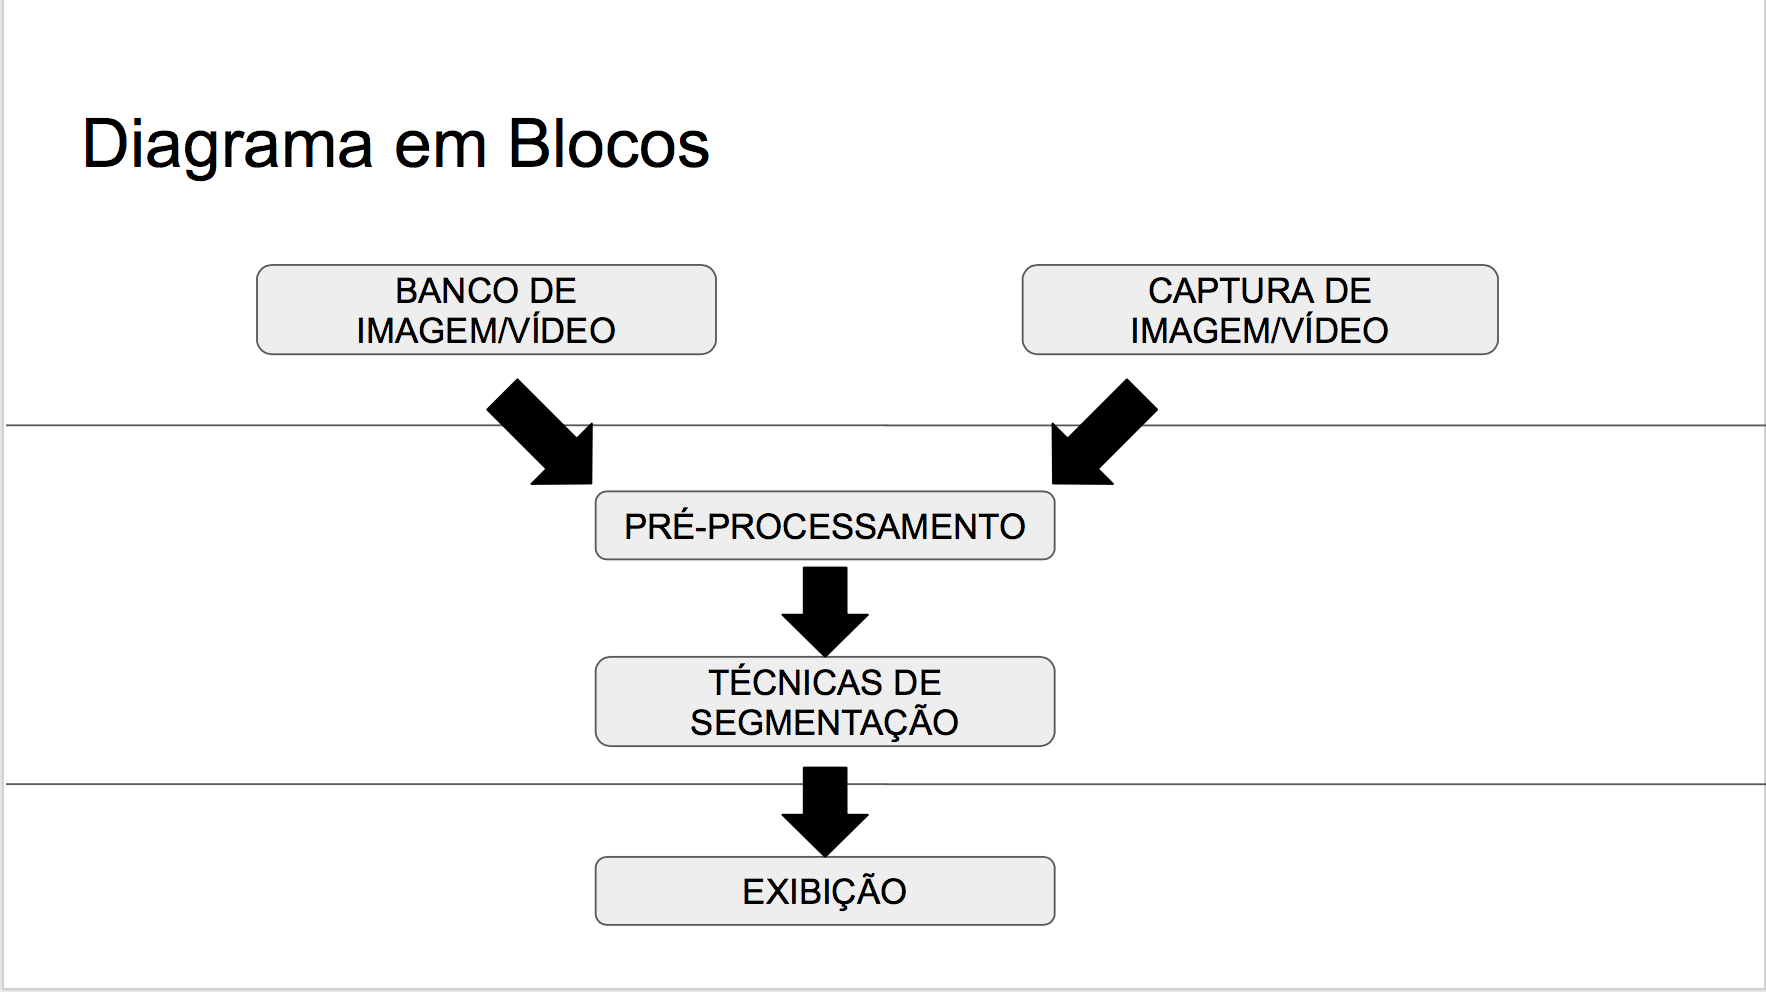
\includegraphics[width=0.7\columnwidth]{img/diag_blocos.png}
           \caption{\label{fig:diag_blocos}Diagrama em Blocos do Projeto.}
           % \vspace{2.0em}
       \end{center}
   \end{figure}
 % Figura -----------------------------------------------------------------------------------------------------------------------------


\section{Justificativa}
Este trabalho pode ser justificado com base nos seguintes pontos:
\begin{itemize}
\item Inexistência de uma solução única para o problema em questão. Trata-se de um problema ainda em aberto com muitas oportunidades a serem exploradas;
\item Diversas aplicações necessitam da segmentação de imagens como parte importante das suas atividades, além de outras que podem ser aprimoradas e desenvolvidas por meio de sua utilização;
\item Visão computacional como domínio promissor da tecnologia, com uma atuação cada vez maior no mercado e interação com outros domínios como robótica e inteligência artificial.
\end{itemize}

\chapter{Segmentação de Imagens}\label{cap:segmentacao}
A segmentação é um problema do tipo "ill-posed" ("mal definido"), uma vez que não existe uma solução única, universal. Por isso, a segmentação é considerada o problema mais difícil de ser resolvido em análise de imagens \citep{Poggio1985}.

\section{Conceito}
A segmentação de imagens tem como uma de suas interpretações como a divisão em regiões ou categorias consideradas "relevantes", que correspondem a objetos ou partes de objetos. Decidir o que é relevante em uma imagem depende do problema a ser resolvido, em que os objetos segmentados devem corresponder às áreas de interesse da aplicação. Dentre essas aplicações, podemos citar os seguintes exemplos:

\begin{itemize}
\item Aplicações militares: Reconhecimento de alvos terrestres, aéreos e navais;
\item Análise de imagens médicas: Identificação de doenças como tumores;
\item Veículos autônomos;
\item Robótica.
\end{itemize}

\section{Segmentação para seres humanos e para computadores}\label{sec:segmenthm}
Para seres humanos, a identificação de regiões similares ou objetos diferentes presentes em uma imagem é um processo fácil. Nosso sistema cognitivo auxiliado por nosso sistema visual nos permite reconhecer e segmentar os objetos de forma instantânea sem nos darmos conta desse processo. Além disso, usamos a segmentação por distância como técnica auxiliar , uma vez que nossa visão estereoscópica nos fornece informação de profundidade.
No caso de computadores, essa tarefa se torna mais complexa, pois envolve a análise de características de cada pixel ou da distribuição da população de pixels. Para isso, deve-se implementar algoritmos de segmentação, os quais serão explorados com maior profundidade nas seções subsequentes dessa pesquisa. A Figura \ref{fig:Berkeley_mulher} exibe uma imagem que foi manualmente segmentada por 4 seres humanos. É possível notar que cada pessoa não identificou como "relevantes" as mesmas áreas, conforme ilustrado pela Figura \ref{fig:Berkeley_mulher_segmentada}. 

% Figura 
  \begin{figure}[!htb]
       \begin{center}  
          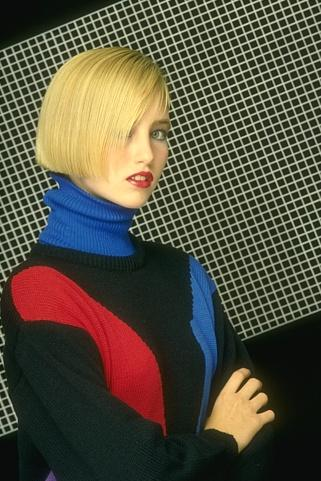
\includegraphics[width=0.3\columnwidth]{img/198023.jpg}
           \caption{\label{fig:Berkeley_mulher}Imagem original\citep{Arbelez2011}.}
           % \vspace{2.0em}
       \end{center}
   \end{figure}

 % Figura 
\begin{figure}[!htb]
 \centering
 \def\baselinestretch{1}\small\normalsize
 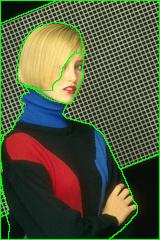
\includegraphics[width=0.2\textwidth]{img/198023-8-color.jpg}\qquad
 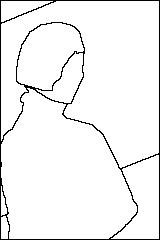
\includegraphics[width=0.2\textwidth]{img/198023-8.jpg}  \qquad
  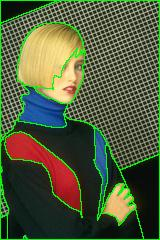
\includegraphics[width=0.2\textwidth]{img/198023-16-color.jpg}  \qquad
 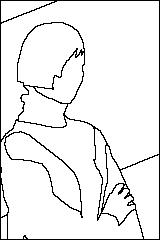
\includegraphics[width=0.2\textwidth]{img/198023-16.jpg}        
 \caption{\label{fig:Berkeley_mulher_segmentada}Imagens segmentadas por seres humanos, gerando 8 e 16 segmentos nas duas primeiras imagens e nas duas últimas, respectivamente.\citep{Arbelez2011}.}
 %\vspace{2.0em}
\end{figure}


% Figura 
\begin{figure}[!h]
 \centering
 \def\baselinestretch{1}\small\normalsize
 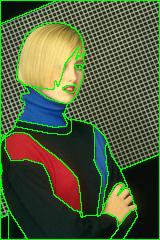
\includegraphics[width=0.2\textwidth]{img/198023-22-color.jpg}\qquad
 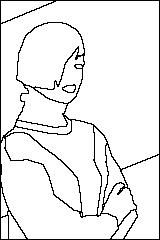
\includegraphics[width=0.2\textwidth]{img/198023-22.jpg}  \qquad
  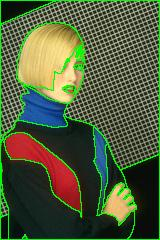
\includegraphics[width=0.2\textwidth]{img/198023-26-color.jpg}  \qquad
 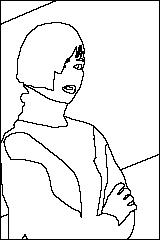
\includegraphics[width=0.2\textwidth]{img/198023-26.jpg}        
 \caption{\label{fig:Berkeley_mulher_segmentada2}Imagens segmentadas por seres humanos, gerando 22 e 26 segmentos nas duas primeiras imagens e nas duas últimas, respectivamente.\citep{Arbelez2011}.}
 %\vspace{2.0em}
\end{figure}




Ainda que o processo de segmentação para humanos seja fácil e automático, é comum e natural que diferentes pessoas identifiquem objetos ou partes de objetos distintos em uma dada imagem. Isso se deve à percepção de relevância atribuída a cada região variar com a interpretação pessoal de cada um. 
O mesmo problema ocorre de forma mais acentuada com relação aos diferentes algoritmos. Cada algoritmo tem a sua própria abordagem para tratar do mesmo problema e, de acordo com sua implementação, leva a diferentes resultados, que podem ser analisados comparativamente. É importante dizer que o mesmo algoritmo pode ser mais ou menos eficiente de acordo com a imagem utilizada como dado de entrada, possibilitando diversos estudos na área como o tema desta pesquisa. A Figura \ref{fig:indio} ilustra este problema\citep{berkeley} . 

% Figura 
  \begin{figure}[!htb]
       \begin{center}  
          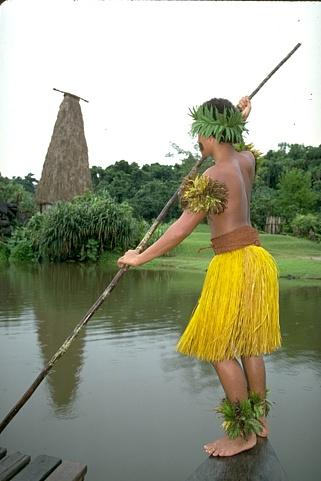
\includegraphics[width=0.3\columnwidth]{img/101087.jpg}
           \caption{\label{fig:indio}Imagem original\citep{berkeley}.}
           % \vspace{2.0em}
       \end{center}
   \end{figure}



 % Figura -----------------------------------------------------------------------------------------------------------------------------       
\begin{figure}[!htb]
 \centering
 \def\baselinestretch{1}\small\normalsize
 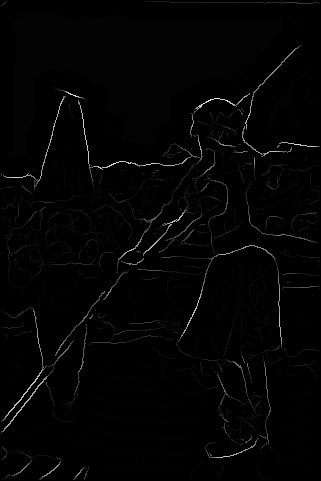
\includegraphics[width=0.2\textwidth]{img/101087-77.jpg}\qquad
 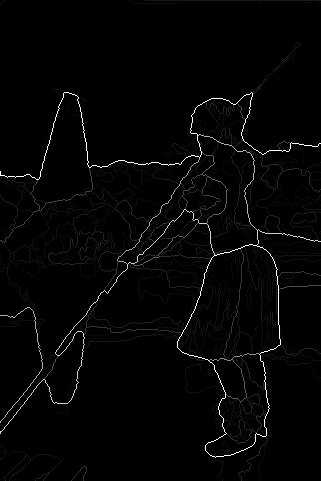
\includegraphics[width=0.2\textwidth]{img/101087-80.jpg}  \qquad 
  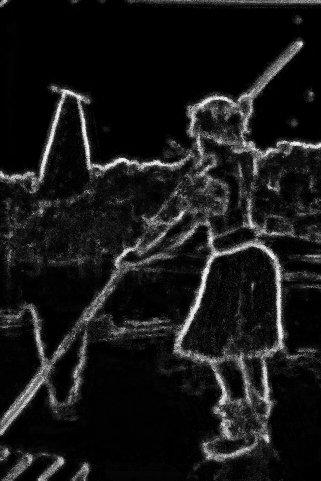
\includegraphics[width=0.2\textwidth]{img/101087-82.jpg}  \qquad
 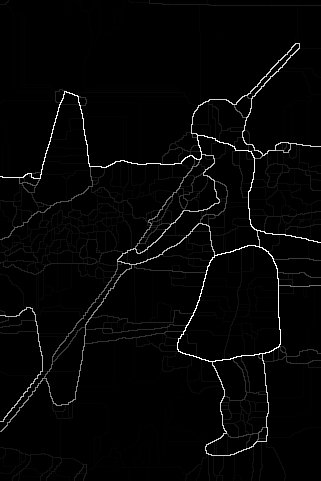
\includegraphics[width=0.2\textwidth]{img/101087-85.jpg}        
 \caption{\label{fig:indiosegmentado}Resultados de 4 algoritmo de detec\c{c}\~{a}o de bordas \citep{berkeley}.}
 %\vspace{2.0em}
\end{figure}
 % Figura -----------------------------------------------------------------------------------------------------------------------------



Devido a  grande variedade de algoritmos existentes, nos limitaremos à explicação dos principais e mais utilizados, os quais fornecem um bom entendimento das técnicas utilizadas e servem como base para o desenvolvimento de novas técnicas. O Capitulo \ref{cap:algoritmos} apresenta as técnicas estudadas.



\chapter{Algoritmos de Segmentação}\label{cap:algoritmos}

Este capitulo descreve 4 técnicas de segmentação de imagens, sendo a por limiar (Thresholding) a mais simples. As técnicas baseadas em bordas e regiões são mais complexas e demandam um ônus computacional mais elevado.

% \section{Tipos de Algoritmos}
\begin{itemize}
    \item Thresholding
    \item Método Baseado em Bordas 
    \item Método Baseado em Regiões
    \begin{itemize}  
        \item Split and Merge
        \item Watershed
    \end{itemize}
\end{itemize}

\subsection{Thresholding}
É o método mais simples de segmentação de imagens.
Busca dividir a imagem em duas categorias: objetos (foreground) e plano de fundo (background). 
Cada pixel é alocado a uma categoria de acordo com seu valor em níveis de cinza.

Dado um limiar T (threshold), o pixel com valor $f_i_j$  e localizado na posição (i,j)  é alocado à:
\\
\begin{cases}
$  categoria 1, se: f_{ij} $\leq$ T. $ \\
$  categoria 2, caso contrário. $ \\
\end{cases}
\\
O limiar T pode ser escolhido manualmente, tentando diferentes valores de T e analisando qual deles é mais eficiente na identificação dos objetos de interesse.
O threshold T também pode ser escolhido a partir do Histograma da imagem, e escolhe-se T como o valor entre as duas distribuições de cinza.

A seguir há a figura \ref{fig:einstein}, uma imagem original do Einstein,  e as duas formas de segmentação de imagens por limiar (thresholding). Enquanto na figura \ref{fig:einsteinglobal} há um limiar T fixo , na  figura \ref{fig:einsteinlocal} ele é variável.

\subsection*{Threshold Global}
O mesmo valor de T é usado para a imagem inteira.

% Figura 
  \begin{figure}[!htb]
       \begin{center}  
          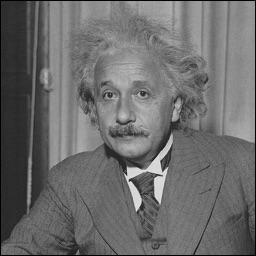
\includegraphics[width=0.3\columnwidth]{img/einstein.jpg}
           \caption{\label{fig:einstein}Imagem original\citep{stanford}.}
           % \vspace{2.0em}
       \end{center}
   \end{figure}

% Figura 
  \begin{figure}[!htb]
       \begin{center}  
          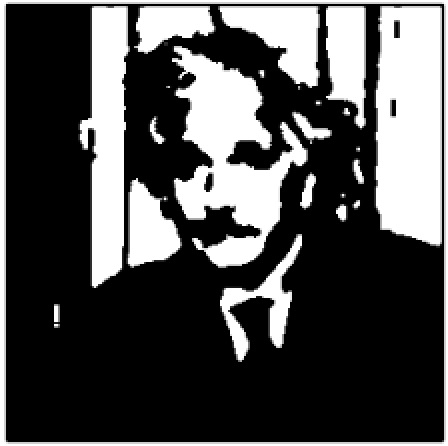
\includegraphics[width=0.3\columnwidth]{img/einstein-globalthresholding127.jpg}
           \caption{\label{fig:einsteinglobal}Imagem segmentada pelo algoritmo threshold global.}
           % \vspace{2.0em}
       \end{center}
   \end{figure}

\subsection*{Threshold Local (ou dinâmico)}
Divide-se a imagem em regiões distintas e adota-se um valor T para cada uma delas, onde esse valor funcionará como threshold local. 

% Figura 
  \begin{figure}[!htb]
       \begin{center}  
          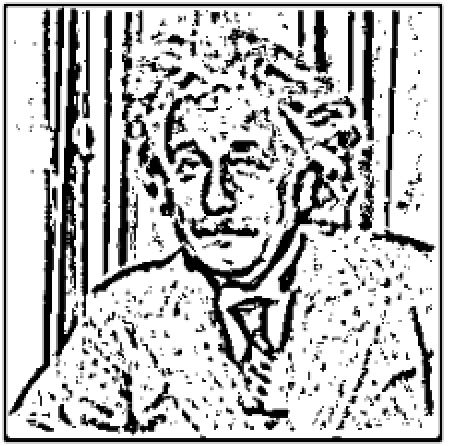
\includegraphics[width=0.3\columnwidth]{img/einstein-localthresholding-adaptivegausian.jpg}
           \caption{\label{fig:einsteinlocal}Imagem segmentada pelo método de segmentação thresholding local, chamado de adaptive gaussian  thresholding.}
           % \vspace{2.0em}
       \end{center}
   \end{figure}
   
   Pode-se observar pela figura \ref{fig:einsteinlocal} que houve a separação em mais regiões nesse método do que na figura \ref{fig:einsteinglobal}, já que foi usado um limiar mais apropriado a cada região.

\subsection{Baseado em Bordas}
Primeiramente, classifica-se os pixels como “borda” ou “não-borda”.
Depois, divide-se a imagem em regiões, baseado nas bordas detectadas.

As bordas são identificadas por meio das descontinuidades, isto é, variações abruptas nos valores dos pixels. 

Como pode-se perceber na figura \ref{fig:smandrill}, por esse método houve a segmentação da imagem de um macaco em regiões de olhos, nariz e outras partes. 

% ------------------------------------------------------------------------------------------------------------
% Figura 
\begin{figure}[!htb]
 \centering
 \def\baselinestretch{1}\small\normalsize
 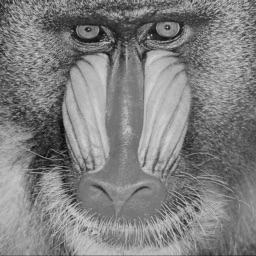
\includegraphics[width=0.4\textwidth]{img/stf-smandrill.jpg}\qquad
 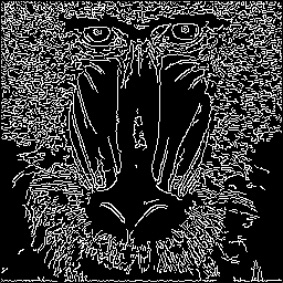
\includegraphics[width=0.4\textwidth]{img/stf-smandrill-edgedetect.jpg} 
 \caption{\label{fig:smandrill} Uma imagem de um macaco \citep{stanford} à esquerda e à direita segmentada pelo método de detecção de bordas em linguagem de programação python.}
 %\vspace{2.0em}
\end{figure}


\subsection{Baseado em Regiões}
\subsubsection*{O que é uma região?}
Uma região pode ser “definida” como um grupo de pixels conectados com propriedades similares.

Porém, é um conceito importante e difícil de definir, já que depende da interpretação do que seria uma região  em determinado caso.

Pelas figuras da seção \ref{sec:segmenthm} do capitulo \ref{cap:segmentacao}, nota-se as diferentes interpretações do conceito de região pelas diferentes quantidades de regiões notadas por humanos nas Figuras \ref{fig:Berkeley_mulher_segmentada} e \ref{fig:Berkeley_mulher_segmentada2}. Tal fato também acontece com os computadores, como nota-se pelas figuras \ref{fig:indiosegmentado}.

\subsubsection{Split and Merge}
\subsubsection*{Procedimento}
As etapas fundamentais deste algoritmo segundo  são: 
\begin{enumerate}
    \item Criar critério para definir o que é uma área homogênea.
    \item Começar com a imagem completa e divide em 4 sub-imagens.
    \item Checar cada sub-imagem e dividi-la novamente em 4 novas sub-imagens caso ela não seja homogênea.
    \item Repetir Passo 3 até que não se consiga mais subdividir.
    \item Comparar sub-imagens com suas regiões vizinhas e agrupá-las se forem homogêneas.
    \item Repetir Passo 5 até que não se consiga mais agrupar.
\end{enumerate}

\subsubsection*{EXEMPLO - QUADTREE}
Um exemplo de segmentação baseada em região Split and Merge é o algoritmo quadtree. A figura \ref{fig:aral} abaixo ilustra a segmentação de imagem por este algoritmo, e observa-se a segmentação da região que contém água na figura.

% ------------------------------------------------------------------------------------------------------------
% Figura 
\begin{figure}[!htb]
 \centering
 \def\baselinestretch{1}\small\normalsize
 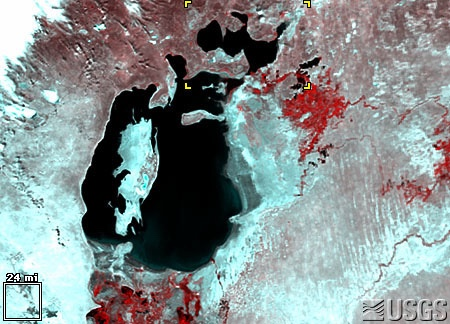
\includegraphics[width=0.4\textwidth]{img/stf-aral1997.jpg}\qquad
 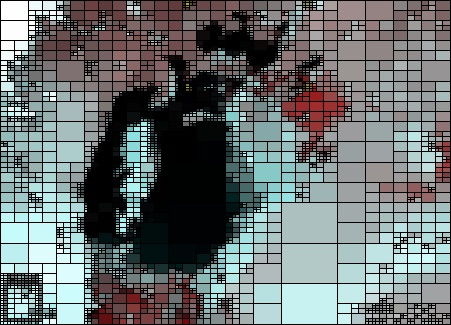
\includegraphics[width=0.4\textwidth]{img/stf-aral1997-quadtree.jpg} 
 \caption{\label{fig:aral}Uma representação visual de uma região \citep{stanford} à esquerda e à direita segmentada pelo algoritmo quadtree em linguagem de programação python.}
 %\vspace{2.0em}
\end{figure}

\subsubsection{Region growing (abordagem bottom-up)}
\subsubsection*{Procedimento}
As etapas fundamentais deste algoritmo são: 
\begin{enumerate}
    \item Identificar o ponto de partida.
    \item Incluir pixels vizinhos com características similares (nível de cinza, textura, cor, etc).
    \item Continuar até que todos os pixels estejam associados com um dos pontos de partida.
\end{enumerate}

\subsubsection*{EXEMPLO - WATERSHEED}
Um exemplo de segmentação baseada no método Region growing é o algoritmo watershed. A figura \ref{fig:coins} abaixo ilustra a segmentação de imagem por este algoritmo, e observa-se regiões distintas correspondentes à cada moeda da figura.

% ------------------------------------------------------------------------------------------------------------
% Figura 
\begin{figure}[!htb]
 \centering
 \def\baselinestretch{1}\small\normalsize
 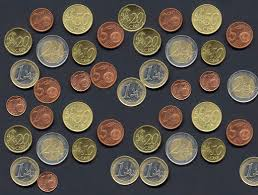
\includegraphics[width=0.4\textwidth]{img/stf-coins.jpg}\qquad
 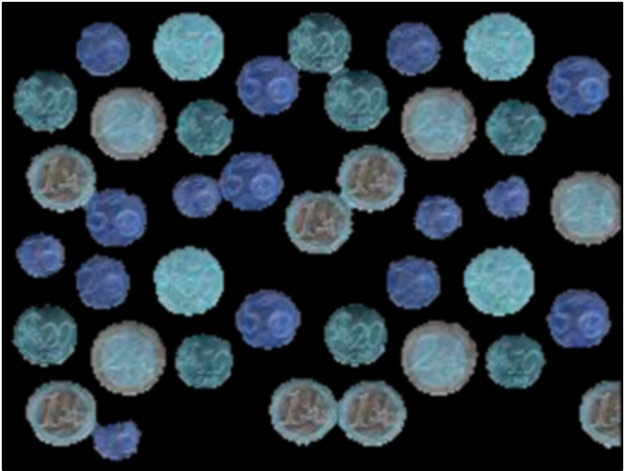
\includegraphics[width=0.4\textwidth]{img/stf-coins-watersheed.jpg} 
 \caption{\label{fig:coins}Imagem de uma moeda \citep{stanford} à esquerda e à direita segmentada pelo algoritmo watersheed em linguagem de programação python.}
 %\vspace{2.0em}
\end{figure}
 
% Stanford DataSet
%  https://scien.stanford.edu/index.php/test-images-and-videos/
 


\chapter{Ferramentas}

\section{Android Studio}
Plataforma de desenvolvimento de aplicativos para sistemas Android. Criado especificamente para esse propósito, a IDE oficial do Android oferece diversos recursos que aceleram o desenvolvimento e aumentam a qualidade dos aplicativos criados.

Tais recursos como ferramentas de edição, depuração, testes e geração de perfis de código motivaram a escolha dessa plataforma para o desenvolvimento da aplicação dessa pesquisa. Além da programação na linguagem Java, é permitido o desenvolvimento em linguagem nativa, C/C++, por meio da ferramenta Android NDK, que será utilizada na implementação dos algoritmos de segmentação presentes nessa aplicação\citep{androidstudio}.



\section{OpenCV}
Biblioteca open source para o desenvolvimento de aplicativos na área de Visão Computacional. Conta com mais de 2500 algoritmos otimizados com abordagens clássicas e no estado da arte nas áreas de visão computacional e aprendizado de máquina, sendo, portanto, uma ferramenta amplamente usada em aplicações que envolvem o processamento de imagens (mais de 14 milhões de downloads). Tem interfaces para linguagens como C++, C, Python e Java e suporta diferentes plataformas como Windows, Linux, Mac OS e Android. A maior performance é obtida com seu uso em C++ pelo fato de ser sua linguagem nativa.\citep{opencv}

\section{Android NDK}
O Android Native Developmentt Kit (NDK) é um conjunto de ferramentas que permite a codificação de arquivos de projeto em linguagens nativas como C/C++. Como dito anteriormente, essa ferramenta auxiliará na implementação dos algoritmos de segmentação de imagens que farão parte de nossa aplicação.\citep{ndk}


\chapter{Cronograma}
\section{Definição de Etapas}
\subsection{Escolha do Tema e Estudo de Viabilidade}
A escolha do tema foi a primeira etapa do projeto. O uso de dispositivos móveis, bem como de suas respectivas câmeras tem sido cada dia mais frequentes. Essas câmeras captam informações do ambiente que os cercam e a segmentação de imagem pode ser usado no processamento de imagens de forma a desenvolver soluções computacionalmente automatizáveis.

Após a escolha do tema, foi feito o estudo de viabilidade, de forma a se verificar a possibilidade da cumprimento do objetivo do tema em tempo aceitável.

\subsection{Revisão Bibliográfica}
Rêferencias tais como livros, artigos e outras referências foram estudadas durante o período de revisão bibliográfica, de forma a permitir um embasamento bibliográfico do projeto.

\subsection{Elaboração da Monografia}
Esta fase do projeto se estende até o termino do projeto de fim de curso. Nesta última, confecciona-se um relatório utilizando-se os conhecimentos adquiridos desde o início do projeto.

\subsection{Estudo e Análise dos Algoritmos de Segmentação de Imagem}
Na aplicação proposta, alguns algoritmos de segmentação de imagem serão implementados no dispositivo móvel, de modo a estudá-los e verificar o mais apropriado à aplicação.

\subsection{Implementação}
A implementação ocorrerá após o estudo dos algoritmos e da definição de quais deles são mais indicados à proposta. Em uma primeira fase os algoritmos serão implementados em outros ambientes de desenvolvimento e em uma segunda etapa será realizada a portabilidade para o ambiente Android.

\subsection{Teste}
Os testes com as imagens em diferentes algoritmos serão realizados e, com a implementação pronta, pode-se observar e comparar os resultados dos algoritmos.

\subsection{Entrega do Relatório Final e Apresentação}
A partir das análises e de todo conteúdo, implementação, análises e testes, será feito o relatório e a apresentação à banca.


\section{Entregáveis}
Os entregáveis serão:

\begin{itemize}
\item Projeto do  Aplicativo
\item Escolha dos Algoritmos 
\item Aplicativo em Ambiente Android de Segmentação de Imagens implementado
\item Testes e análises comparativas
\end{itemize}

%Os dois primeiros ítens serão entregues durante a apresentação da Verficação Corrente (VC),e os outros serão entregues por ocasião da apresentação da Verificação Final (VF).

\begin{table}[!htpb]
\centering

% definindo o tamanho da fonte para small
% outros possíveis tamanhos: footnotesize, scriptsize
\begin{small} 
  
% redefinindo o espaçamento das colunas
\setlength{\tabcolsep}{3pt} 

% \cline é semelhante ao \hline, porém é possível indicar as colunas que terão essa a linha horizontal
% \multicolumn{10}{c|}{Meses} indica que dez colunas serão mescladas e a palavra Meses estará centralizada dentro delas.

\begin{tabular}{|c|c|c|c|c|c|c|c|c|c|c|}\hline
 & \multicolumn{9}{c|}{Meses}\\ \cline{2-10}
\raisebox{1.5ex}{Etapa} & FEV & MAR & ABR & MAI & JUN & JUL & AGO & SET & OUT \\ \hline

Escolha do Tema e Estudo de Viabilidade & X & X & X & & & & & &   \\ \hline
Revisão Bibliográfica & X & X & X & X & & & & &   \\ \hline
Elaboração da Monografia & X & X & X & X & X & X & X & X & X    \\ \hline
Estudo e Análise dos Algoritmos  & &  &  & &  & X & X & X &  \\ 
de Segmentação de Imagem & &  &  & &  &  &  &  &  \\ \hline
Implementação & &  &  & &  & X & X & X &    \\ \hline
Teste & & & & & & & & X &   \\ \hline
Entrega do Relatório Final e Apresentação & & & & & & & & & X  \\ \hline

\end{tabular} 
\end{small}
\caption{Cronograma das atividades previstas}
\label{t_cronograma}
\end{table} 

%\chapter{REFRÊNCIAS BIBLIOGRÁFICAS}
%\begin{itemize}
%    \item GLOCKSTEIN, Bob. Quadtrees and Octrees. Disponível em: <http://euklid.mi.uni-koeln.de/c/mirror/www.cs.curtin.edu.au/units/cg351-551/notes/lect51.html>. Acesso em: 10 mai. 2017
%    \item Chris. Segmentation. Disponível em: <http://www.bioss.ac.uk/people/chris/ch4.pdf>. Acesso em: 10 mai. 2017
%    \item STRAND, Robin. Segmentation. Disponível em: <http://www.it.uu.se/edu/course/homepage/\\bild1/ht14/L6\_segmentation.pdf>. Acesso em: 10 mai. 2017
%\end{itemize}






\chapter{Segmentação de Imagens}\label{cap:segmentacao}
A segmentação é um problema do tipo "\textit{ill-posed}" ("mal definido"), uma vez que não existe uma solução única, universal. Por isso, a segmentação é considerada o problema mais difícil de ser resolvido em análise de imagens \citep{Poggio1985}.

\section{Conceito}
A segmentação de imagens tem como uma de suas interpretações como a divisão em regiões ou categorias consideradas "relevantes", que correspondem a objetos ou partes de objetos. Decidir o que é relevante em uma imagem depende do problema a ser resolvido, em que os objetos segmentados devem corresponder às áreas de interesse da aplicação. Dentre essas aplicações, podemos citar os seguintes exemplos:

\begin{itemize}
\item Aplicações militares: Reconhecimento de alvos terrestres, aéreos e navais;
\item Análise de imagens médicas: Identificação de doenças como tumores;
\item Veículos autônomos; e
\item Robótica.
\end{itemize}

\section{Segmentação para seres humanos e para computadores}\label{sec:segmenthm}
Para seres humanos, a identificação de regiões similares ou objetos diferentes presentes em uma imagem é um processo fácil. Seu sistema cognitivo auxiliado por seu sistema visual permite reconhecer e segmentar os objetos de forma instantânea sem a percepção de todo esse processo. Além disso, o uso da segmentação por distância como técnica auxiliar é outro fator que contribui para esse processo, uma vez que sua visão estereoscópica lhes fornece informação de profundidade.
No caso de computadores, essa tarefa se torna mais complexa, pois envolve a análise de características de cada pixel ou da distribuição da população de pixels. Para isso, deve-se implementar algoritmos de segmentação, os quais serão explorados com maior profundidade nas seções subsequentes dessa pesquisa. A Figura \ref{fig:Berkeley_mulher} exibe uma imagem que foi manualmente segmentada por 4 seres humanos. É possível notar que cada pessoa não identificou como "relevantes" as mesmas áreas, conforme ilustrado pela Figura \ref{fig:Berkeley_mulher_segmentada}. 

% Figura 
  \begin{figure}[!htb]
       \begin{center}  
          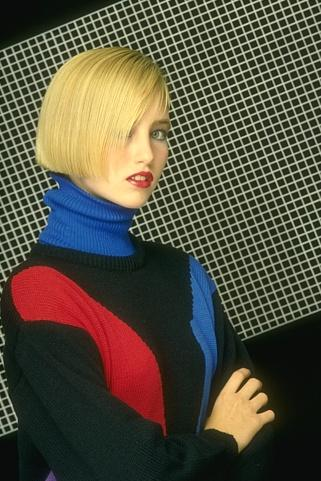
\includegraphics[width=0.3\columnwidth]{img/198023.jpg}
           \caption{\label{fig:Berkeley_mulher}Imagem original\citep{Arbelez2011}.}
           % \vspace{2.0em}
       \end{center}
   \end{figure}

 % Figura 
\begin{figure}[!htb]
 \centering
 \def\baselinestretch{1}\small\normalsize
 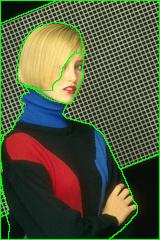
\includegraphics[width=0.2\textwidth]{img/198023-8-color.jpg}\qquad
 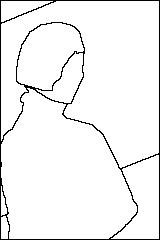
\includegraphics[width=0.2\textwidth]{img/198023-8.jpg}  \qquad
  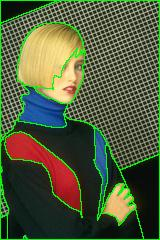
\includegraphics[width=0.2\textwidth]{img/198023-16-color.jpg}  \qquad
 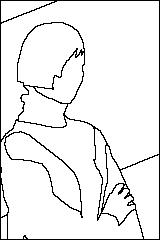
\includegraphics[width=0.2\textwidth]{img/198023-16.jpg}        
 \caption{\label{fig:Berkeley_mulher_segmentada}Imagens segmentadas por seres humanos, gerando 8 e 16 segmentos nas duas primeiras imagens e nas duas últimas, respectivamente.\citep{Arbelez2011}.}
 %\vspace{2.0em}
\end{figure}


% Figura 
\begin{figure}[!h]
 \centering
 \def\baselinestretch{1}\small\normalsize
 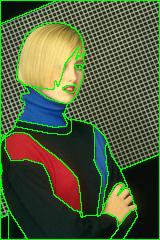
\includegraphics[width=0.2\textwidth]{img/198023-22-color.jpg}\qquad
 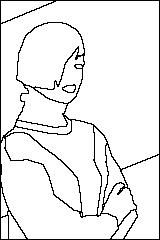
\includegraphics[width=0.2\textwidth]{img/198023-22.jpg}  \qquad
  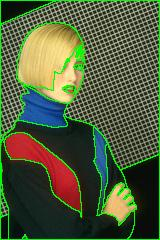
\includegraphics[width=0.2\textwidth]{img/198023-26-color.jpg}  \qquad
 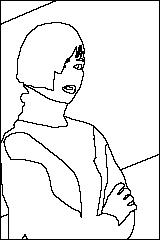
\includegraphics[width=0.2\textwidth]{img/198023-26.jpg}        
 \caption{\label{fig:Berkeley_mulher_segmentada2}Imagens segmentadas por seres humanos, gerando 22 e 26 segmentos nas duas primeiras imagens e nas duas últimas, respectivamente.\citep{Arbelez2011}.}
 %\vspace{2.0em}
\end{figure}




Ainda que o processo de segmentação para humanos seja fácil e automático, é comum e natural que diferentes pessoas identifiquem objetos ou partes de objetos distintos em uma dada imagem. Isso se deve à percepção de relevância atribuída a cada região variar com a interpretação pessoal de cada um. 
O mesmo problema ocorre de forma mais acentuada com relação aos diferentes algoritmos. Cada algoritmo tem a sua própria abordagem para tratar do mesmo problema e, de acordo com sua implementação, leva a diferentes resultados, que podem ser analisados comparativamente. É importante dizer que o mesmo algoritmo pode ser mais ou menos eficiente de acordo com a imagem utilizada como dado de entrada, possibilitando diversos estudos na área como o tema desta pesquisa. A Figura \ref{fig:indio} ilustra este problema\citep{berkeley} . 

% Figura 
  \begin{figure}[!htb]
       \begin{center}  
          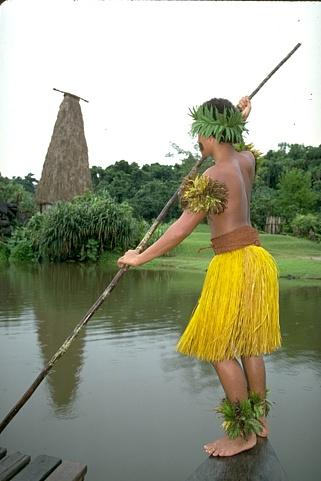
\includegraphics[width=0.3\columnwidth]{img/101087.jpg}
           \caption{\label{fig:indio}Imagem original\citep{berkeley}.}
           % \vspace{2.0em}
       \end{center}
   \end{figure}



 % Figura -----------------------------------------------------------------------------------------------------------------------------       
\begin{figure}[!htb]
 \centering
 \def\baselinestretch{1}\small\normalsize
 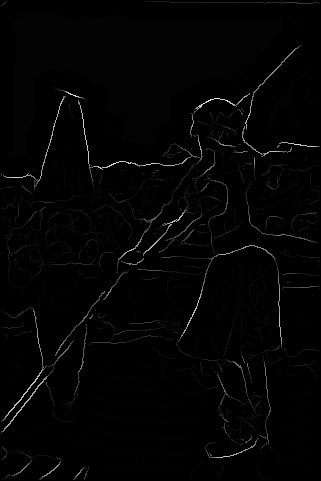
\includegraphics[width=0.2\textwidth]{img/101087-77.jpg}\qquad
 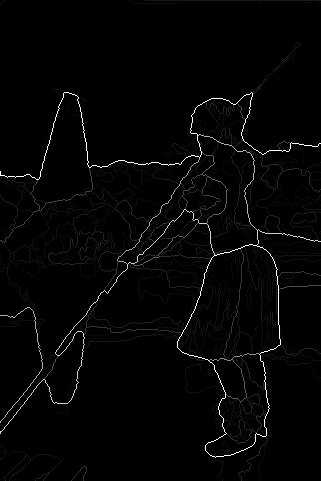
\includegraphics[width=0.2\textwidth]{img/101087-80.jpg}  \qquad 
  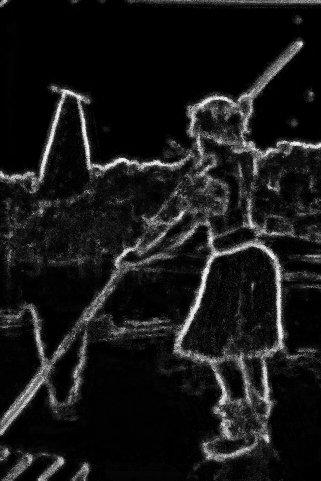
\includegraphics[width=0.2\textwidth]{img/101087-82.jpg}  \qquad
 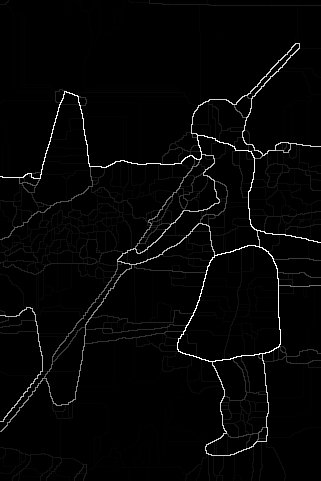
\includegraphics[width=0.2\textwidth]{img/101087-85.jpg}        
 \caption{\label{fig:indiosegmentado}Resultados de 4 algoritmo de detec\c{c}\~{a}o de bordas \citep{berkeley}.}
 %\vspace{2.0em}
\end{figure}
 % Figura -----------------------------------------------------------------------------------------------------------------------------


Devido a grande variedade de algoritmos existentes, essa pesquisa se limitará à explicação dos principais e mais utilizados, os quais fornecem um bom entendimento das técnicas utilizadas e servem como base para o desenvolvimento de novas técnicas.



\chapter{Algoritmos de Segmentação}\label{cap:algoritmos}

Este capítulo descreve 4 técnicas de segmentação de imagens, sendo a por limiar (\textit{thresholding}) a mais simples. As técnicas baseadas em bordas e regiões são mais complexas e demandam um ônus computacional mais elevado.

% \section{Tipos de Algoritmos}
\begin{itemize}
    \item \textit{Thresholding};
    \item Método Baseado em Bordas; e  
    \item Método Baseado em Regiões
    \begin{itemize}  
        \item \textit{Split and Merge}; e
        \item \textit{Watershed}.
    \end{itemize}
\end{itemize}

\subsection{\textit{Thresholding}}\label{sec:alg_thresholding}
É um método simples de segmentação de imagens.
Busca dividir a imagem em duas categorias: objetos (\textit{foreground}) e plano de fundo (\textit{background}). 
Cada \textit{pixel} é alocado a uma categoria de acordo com seu valor em níveis de cinza.

Dado um limiar T (\textit{threshold}), o \textit{pixel} com valor $f_i_j$  e localizado na posição (i,j)  é alocado à:
\\
\begin{cases}
$  categoria 1, se: f_{ij} $\leq$ T. $ \\
$  categoria 2, caso contrário. $ \\
\end{cases}
\\
O limiar T pode ser escolhido manualmente, tentando diferentes valores de T e analisando qual deles é mais eficiente na identificação dos objetos de interesse.
O \textit{threshold} T também pode ser escolhido a partir do histograma da imagem, e escolhe-se T como o valor entre as duas distribuições de cinza.

A seguir há a figura \ref{fig:einstein}, uma imagem original do Einstein,  e as duas formas de segmentação de imagens por limiar (\textit{thresholding}). Enquanto na figura \ref{fig:einsteinglobal} há um limiar T fixo , na  figura \ref{fig:einsteinlocal} ele é variável.

\subsection*{\textit{Threshold} Global}
O mesmo valor de T é usado para a imagem inteira.

% Figura 
  \begin{figure}[!htb]
       \begin{center}  
          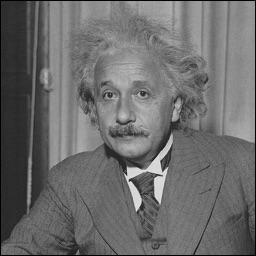
\includegraphics[width=0.3\columnwidth]{img/einstein.jpg}
           \caption{\label{fig:einstein}Imagem original\citep{stanford}.}
           % \vspace{2.0em}
       \end{center}
   \end{figure}

% Figura 
  \begin{figure}[!htb]
       \begin{center}  
          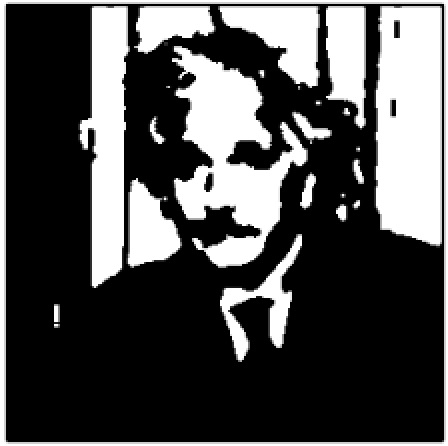
\includegraphics[width=0.3\columnwidth]{img/einstein-globalthresholding127.jpg}
           \caption{\label{fig:einsteinglobal}Imagem segmentada pelo algoritmo threshold global.}
           % \vspace{2.0em}
       \end{center}
   \end{figure}

\subsection*{\textit{Threshold} Local (ou dinâmico)}
Divide-se a imagem em regiões distintas e adota-se um valor T para cada uma delas, onde esse valor funcionará como threshold local. 

% Figura 
  \begin{figure}[!htb]
       \begin{center}  
          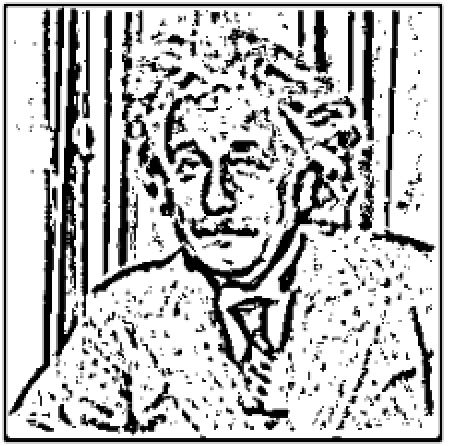
\includegraphics[width=0.3\columnwidth]{img/einstein-localthresholding-adaptivegausian.jpg}
           \caption{\label{fig:einsteinlocal}Imagem segmentada pelo método de segmentação thresholding local, chamado de adaptive gaussian  thresholding.}
           % \vspace{2.0em}
       \end{center}
   \end{figure}
   
   Pode-se observar pela figura \ref{fig:einsteinlocal} que houve a separação em mais regiões nesse método do que na figura \ref{fig:einsteinglobal}, já que foi usado um limiar mais apropriado a cada região.

\subsection{Baseado em Bordas}
Primeiramente, classifica-se os \textit{pixels} como “borda” ou “não-borda”.
Depois, divide-se a imagem em regiões, baseado nas bordas detectadas.

As bordas são identificadas por meio das descontinuidades, isto é, variações abruptas nos valores dos \textit{pixels}. 

Como pode-se perceber na figura \ref{fig:smandrill}, por esse método houve a segmentação da imagem de um macaco em regiões de olhos, nariz e outras partes. 

% ------------------------------------------------------------------------------------------------------------
% Figura 
\begin{figure}[!htb]
 \centering
 \def\baselinestretch{1}\small\normalsize
 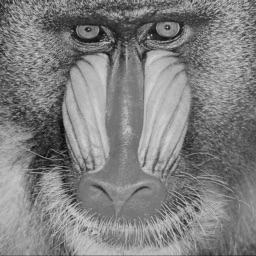
\includegraphics[width=0.4\textwidth]{img/stf-smandrill.jpg}\qquad
 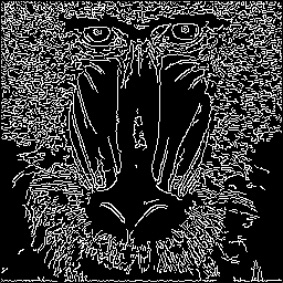
\includegraphics[width=0.4\textwidth]{img/stf-smandrill-edgedetect.jpg} 
 \caption{\label{fig:smandrill} Uma imagem de um macaco \citep{stanford} à esquerda e à direita segmentada pelo método de detecção de bordas em linguagem de programação python.}
 %\vspace{2.0em}
\end{figure}


\subsection{Baseado em Regiões}
\subsubsection*{O que é uma região?}
Uma região pode ser “definida” como um grupo de \textit{pixels} conectados com propriedades similares.

Porém, é um conceito importante e difícil de definir, já que depende da interpretação do que seria uma região  em determinado caso.

Pelas figuras da seção \ref{sec:segmenthm} do capítulo \ref{cap:segmentacao}, nota-se as diferentes interpretações do conceito de região pelas diferentes quantidades de regiões notadas por humanos nas Figuras \ref{fig:Berkeley_mulher_segmentada} e \ref{fig:Berkeley_mulher_segmentada2}. Tal fato também acontece com os computadores, como nota-se pelas figuras \ref{fig:indiosegmentado}.

\subsubsection{\textit{Split and Merge}}
\subsubsection*{Procedimento}
As etapas fundamentais deste algoritmo segundo  são: 
\begin{enumerate}
    \item Criar critério para definir o que é uma área homogênea.
    \item Começar com a imagem completa e divide em 4 sub-imagens.
    \item Checar cada sub-imagem e dividi-la novamente em 4 novas sub-imagens caso ela não seja homogênea.
    \item Repetir Passo 3 até que não se consiga mais subdividir.
    \item Comparar sub-imagens com suas regiões vizinhas e agrupá-las se forem homogêneas.
    \item Repetir Passo 5 até que não se consiga mais agrupar.
\end{enumerate}

\subsubsection*{EXEMPLO - \textit{QUADTREE}}
Um exemplo de segmentação baseada em região Split and Merge é o algoritmo quadtree. A figura \ref{fig:aral} abaixo ilustra a segmentação de imagem por este algoritmo, e observa-se a segmentação da região que contém água na figura.

% ------------------------------------------------------------------------------------------------------------
% Figura 
\begin{figure}[!htb]
 \centering
 \def\baselinestretch{1}\small\normalsize
 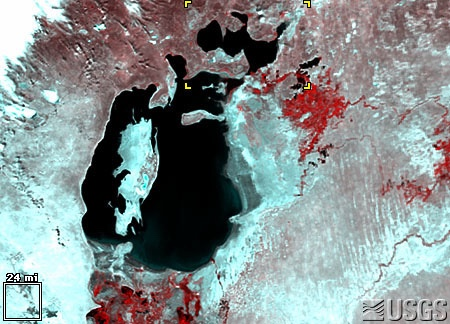
\includegraphics[width=0.4\textwidth]{img/stf-aral1997.jpg}\qquad
 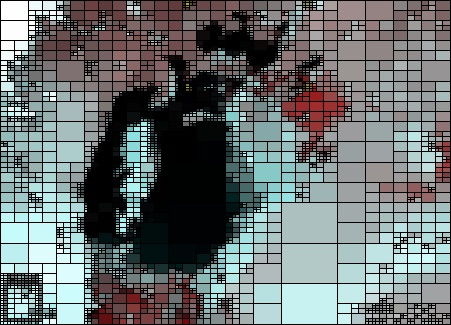
\includegraphics[width=0.4\textwidth]{img/stf-aral1997-quadtree.jpg} 
 \caption{\label{fig:aral}Uma representação visual de uma região \citep{stanford} à esquerda e à direita segmentada pelo algoritmo quadtree em linguagem de programação python.}
 %\vspace{2.0em}
\end{figure}

\subsubsection{\textit{Region growing} (abordagem \textit{bottom-up})}
\subsubsection*{Procedimento}
As etapas fundamentais deste algoritmo são: 
\begin{enumerate}
    \item Identificar o ponto de partida.
    \item Incluir \textit{pixels} vizinhos com características similares (nível de cinza, textura, cor, etc).
    \item Continuar até que todos os \textit{pixels} estejam associados com um dos pontos de partida.
\end{enumerate}

\subsubsection*{EXEMPLO - \textit{WATERSHED}}
Um exemplo de segmentação baseada no método \textit{Region growing} é o algoritmo \textit{watershed}. A figura \ref{fig:coins} abaixo ilustra a segmentação de imagem por este algoritmo, e observa-se regiões distintas correspondentes à cada moeda da figura.

% ------------------------------------------------------------------------------------------------------------
% Figura 
\begin{figure}[!htb]
 \centering
 \def\baselinestretch{1}\small\normalsize
 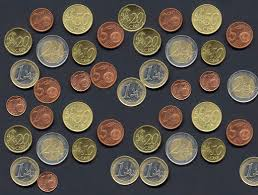
\includegraphics[width=0.4\textwidth]{img/stf-coins.jpg}\qquad
 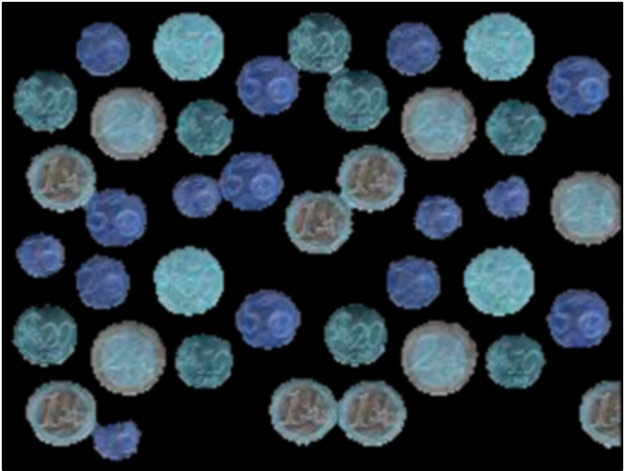
\includegraphics[width=0.4\textwidth]{img/stf-coins-watersheed.jpg} 
 \caption{\label{fig:coins}Imagem de uma moeda \citep{stanford} à esquerda e à direita segmentada pelo algoritmo watersheed em linguagem de programação python.}
 %\vspace{2.0em}
\end{figure}
 
% Stanford DataSet
%  https://scien.stanford.edu/index.php/test-images-and-videos/
 


\chapter{Algoritmo \textit{watershed} Adaptado}\label{cap:algoritmo}

O algoritmo proposto nessa pesquisa é baseado no algoritmo "\textit{Watershed Algorithm Based On Connected Components}", apresentado em \cite{ruparelia2012implementation}, o qual trata-se de uma variação da técnica de \textit{watershed} com resultados de segmentação considerados satisfatórios além da menor complexidade computacional com relação à abordagem tradicional \textit{watershed}.

\section{\textit{Watershed}}\label{sec:watershed}
\textit{Watershed} é uma técnica de segmentação eficiente e poderosa. Tal técnica tem a tendência de gerar sempre resultados com contornos fechados e bem definidos, o que é de grande importância para o processo de segmentação de imagens. Além disso, comparada a outras técnicas de segmentação, apresenta menor complexidade computacional.

Duas abordagens são utilizadas para explicar a ideia básica do \textit{watershed} na segmentação de imagens. 
A primeira, denominada "\textit{flooding based watershed}", trata a imagem em níveis de cinza com uma paisagem formada por vales, onde encontram-se os mínimos locais. Considerando um processo de inundação com a água subindo a partir de cada um dos vales, serão construídas barragens nos pontos de encontro da água oriunda de dois vales distintos, chamadas de \textit{watersheds}. Essas barragens, portanto, são interpretadas como bordas entra diferentes regiões da imagem.\citep{l6} 

% Figura
	\begin{figure}[!htb]
       \begin{center}  
          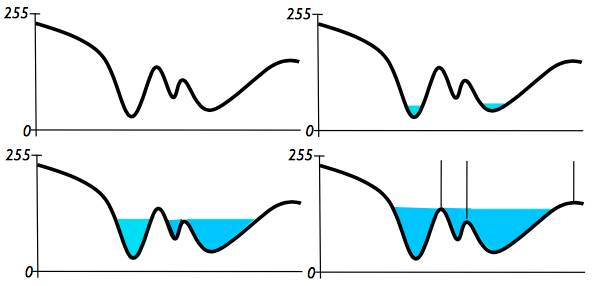
\includegraphics[width=0.6\columnwidth]{img/abordagem_flooding.jpg}
           \caption{\label{fig:abordagem_flooding}Abordagem "\textit{flooding based watershed}".\cite{regseg1}}
           % \vspace{2.0em}
       \end{center}
   \end{figure} 


A outra abordagem, denominada "\textit{rainfalling based watershed}" trata a imagem em níveis de cinza da mesma forma que a primeira, porém o fluxo de água ocorre a partir de gotas de água que ao incidirem em qualquer ponto da superfície escorrerão para um determinado vale, onde encontra-se um mínimo local. O conjunto de pontos para os quais a gota de água escorre para o mesmo local é interpretada como uma região e os limites entre duas regiões adjacentes,  interpretados como bordas, são as \textit{watersheds}. \citep{l6} 

% Figura 
	\begin{figure}[!htb]
       \begin{center}  
          \includegraphics[width=0.6\columnwidth]{img/abordagem_rainfalling.jpg}
           \caption{\label{fig:abordagem_rainfalling}Abordagem "\textit{rainfalling based watershed}". \cite{ruparelia2012implementation}}
           % \vspace{2.0em}
       \end{center}
   \end{figure} 
	

Ambas abordagens tratam da mesma ideia básica da técnica, sendo duas formas diferentes de ilustrar seus funcionamento sobre os quais diferentes algoritmos são propostos.

Um dos principais problemas relacionados à abordagem tradicional do \textit{watershed} é o problema de \textit{over-segmentation}. Para reduzir esse problema, diversas variações de algoritmos baseados na técnica de \textit{watershed} foram implementados, tal qual o algoritmo utilizado nessa pesquisa, explicado detalhadamente na seção \ref{sec:alg} do capítulo \ref{cap:algoritmo}. 

Assim as diferenças entre o algoritmo proposto e o tradicional, como o implementado na biblioteca OpenCV, apresentada na seção \ref{sec:opencv} do anexo 1, conduzirão a uma análise comparativa entre os resultados obtidos por meio de cada um deles.

\section{\textit{Watershed Algorithm Based On Connected Components}}
A análise comparativa dos algoritmos \textit{watershed} baseado em componentes conectados e \textit{watershed} tradicional permite verificar a maior eficiência do primeiro devido `as seguintes características:

% \section{Características}
\begin{itemize}
    \item Fila FIFO ao invés de fila hierárquica - algoritmo tradicional - que requer sequências de acesso à memória não uniformes;
    \item Estrutura de dados mais simples; e
    \item Menor tempo de execução.
\end{itemize}    

Este algoritmo tem como princípio conectar cada \textit{pixel} (componente), caso este não seja o mínimo local, ao menor \textit{pixel} vizinho. Todos os \textit{pixels} direcionados para o mesmo mínimo local formam um segmento e são, portanto, rotulados da mesma forma.

% Figura
	\begin{figure}[!htb]
       \begin{center}  
          \includegraphics[width=0.9\columnwidth]{img/connected_components.jpg}
           \caption{\label{fig:connected_components}Ilustração do funcionamento da técnica \textit{Watershed Based On Connected Components}. \cite{ruparelia2012implementation}}
           % \vspace{2.0em}
       \end{center}
   \end{figure}

\section{Implementação do Algoritmo}\label{sec:alg}

O algoritmo de segmentação proposto nessa pesquisa, assim como os demais algoritmos baseados na técnica de segmentação por \textit{watershed}, segue a estrutura apresentada na figura \ref{fig:diagrama_blocos_algoritmo}. A imagem original passa por uma etapa de pré-processamento, em que diferentes procedimentos são realizados. Após a etapa de pré-processamento, a imagem é segmentada pela técnica \textit{watershed} e seu resultado pode ser processado, na etapa de pós-processamento, a fim de corrigir algumas falhas geradas pelo processo de segmentação para, finalmente, obter a segmentação como resultado final.
Todas as etapas serão explicadas nas próximas seções de acordo como foram implementadas no algoritmo proposto por essa pesquisa.

% Figura
	\begin{figure}[!htb]
       \begin{center}  
          \includegraphics[width=0.7\columnwidth]{img/diagrama_blocos_algoritmo.jpg}
           \caption{\label{fig:diagrama_blocos_algoritmo}Diagrama de blocos do algoritmo de segmentação dessa pesquisa.}
           % \vspace{2.0em}
       \end{center}
   \end{figure} 

\subsection{Pré-Processamento}
A etapa de pré-processamento tem como objetivo preparar a imagem que será utilizada na segmentação efetivamente. Para isso alguns procedimentos são realizados com o objetivo de retirar ruídos e realçar bordas para facilitar o processo de segmentação a fim de obter um resultado mais eficiente. Além disso, assim como a etapa de pós-processamento, esta etapa visa diminuir o problema de \textit{over-segmentation}, o qual tende a ocorrer quando aplica-se a técnica de \textit{watershed}.
A ordem em que esses procedimentos ocorrem nesta etapa consta na estrutura apresentada pela figura \ref{fig:diagrama_blocos_preprocessamento}.

% Figura
	\begin{figure}[!htb]
       \begin{center}  
          \includegraphics[width=0.8\columnwidth]{img/diagrama_blocos_preprocessamento.jpg}
           \caption{\label{fig:diagrama_blocos_preprocessamento}Diagrama de blocos da etapa de pré-processamento.}
           % \vspace{2.0em}
       \end{center}
   \end{figure}
\clearpage   

\subsubsection{Conversão para Cinza}
Um dos procedimentos realizados na etapa de pré-processamento é a conversão da imagem original colorida para a imagem em níveis de cinza. Utiliza-se a quantização em 256 níveis de cinza (8 bits), onde o nível zero representa o preto e o nível 255, o branco.
O objetivo dessa conversão é tratar a imagem em um canal já que o escopo da presente pesquisa é tratar imagens em escala de cinza.

\subsubsection{Filtro Bilateral}
O filtro biltateral é utilizado como um dos primeiros procedimentos da etapa de pré-processamento a fim de reduzir os ruídos presentes na imagem a ser segmentada, preservando suas bordas.

Abaixo a definição matemática do Filtro Bilateral:

% Figura
	\begin{figure}[!htb]
       \begin{center}  
          \includegraphics[width=0.8\columnwidth]{img/definicao_matematica_filtro_bilateral.jpg}
           \caption{\label{fig:definicao_matematica_filtro_bilateral}Definição matemática do Filtro Bilateral. \citep{Banterle2012}}
           % \vspace{2.0em}
       \end{center}
   \end{figure}
	\clearpage
%\subsubsection{Operador \textit{Not}}
%O operador not é utilizado no pré-processamento para que o algoritmo \textit{watersheed } seja executado da maneira correta, isto é, dos plateaus para os mínimos locais através. Ele inverte cada bit de um \textit{array}.
\subsubsection{Operador Sobel}
O operador Sobel é um operador de detecção de bordas que se baseia no operador gradiente.
Os gradientes horizontal, \textit{Gx}, e vertical, \textit{Gy}, são calculados considerando uma janela de tamanho 3, isto é, \textit{3 x 3 pixels}, e calcula-se uma aproximação do gradiente em cada ponto da seguinte forma: \citep{sobel}

Abaixo a definição matemática do operador Sobel:
% Figura
	\begin{figure}[!htb]
       \begin{center}  
          \includegraphics[width=0.7\columnwidth]{img/definicao_matematica_sobel.jpg}
           \caption{\label{fig:definicao_matematica_sobel}Definição matemática do Operador Sobel.}
           % \vspace{2.0em}
       \end{center}
   \end{figure} 
%\clearpage     
   
Abaixo um exemplo prático da aplicação do operador Sobel:   
% Figura 
\begin{figure}[!htb]
 \centering
 \def\baselinestretch{1}\small\normalsize
 \includegraphics[width=0.4\textwidth]{img/lena_original.png}\qquad
 \includegraphics[width=0.4\textwidth]{img/lena_sobel.png} 
 \caption{\label{fig:lena_sobel}Resultado prática da aplicação do operador Sobel.}
 %\vspace{2.0em}
\end{figure} 
\clearpage

% Equação
%\[G = |G_{x}| + |G_{y}|\]

% Código

%\subsubsection{Filtro de Mediana}
%O objetivo do filtro de mediana é a redução ou, até mesmo, a remoção de ruídos das imagens, a fim de suavizá-las e torná-las mais tratáveis para o processo de segmentação. O filtro de mediana é eficaz para o tratamento de ruídos impulsivos, como o ruído Gaussiano (aleatório) e, principalmente, o ruído sal e pimenta, em que os \textit{pixels} ruidosos assumem os valores máximos e mínimos da imagem.
%Para a implementação do filtro de mediana, considera-se uma imagem com \textit{n x m pixels} e um filtro com janela de \textit{k x k pixels}, onde \textit{k < n e k < m}. Em casa janela considerada na imagem, o valor de cada \textit{pixel} é substituído pelo valor da mediana da mesma janela. No algoritmo, usa-se \textit{k = 3} e o funcionamento do filtro pode ser entendido na figura \ref{fig:filtromediana}.

% Figura
	%\begin{figure}[!htb]
     %  \begin{center}  
      %    \includegraphics[width=0.8\columnwidth]{img/filtromediana.jpg}
       %    \caption{\label{fig:filtromediana}Ilustração do funcionamento do filtro de mediana. \cite{ruparelia2012implementation}}
           % \vspace{2.0em}
       %\end{center}
  % \end{figure}
   
% Código

\subsubsection{Operadores Morfológicos}
Após a aplicação de um detector de bordas, como o operador Sobel, a imagem pode ficar com bordas "falhadas". Como a técnica de \textit{watershed} requer que as regiões estejam "fechadas", ou seja, sem falhas nas bordas, é aplicado um conjunto de operações morfológicas para conectar estas regiões fragmentadas. 
Existem duas operações morfológicas básicas:
% \section{Operações morfológicas básicas}
\begin{itemize}
    \item Erosão; e
    \item Dilatação.
\end{itemize}    

A biblioteca OpenCV fornece 5 transformações morfológicas baseadas nessas duas operações básicas:
% \section{Transformações morfológicas}
\begin{itemize}
    \item \textit{Opening};
    \item \textit{Closing};
    \item \textit{Morphological Gradient};
    \item \textit{Top Hat}; e 
    \item \textit{Black Hat}.
\end{itemize} 
\clearpage


No algoritmo utiliza-se apenas a transformação do gradiente morfológico - \textit{Morphological Gradient} -, a qual é a diferença entre a dilatação e a erosão de uma imagem. Essa transformação é útil para encontrar o contorno de um objeto em uma dada imagem. \citep{morphology_transformations}
% Equação
\[dst = morph_{grad}( src, element ) = dilate( src, element ) - erode( src, element )\]

Abaixo um exemplo prático da aplicação do operador morfológico: 
% Figura 
\begin{figure}[!htb]
 \centering
 \def\baselinestretch{1}\small\normalsize
 \includegraphics[width=0.4\textwidth]{img/org.png}\qquad
 \includegraphics[width=0.4\textwidth]{img/op_morf.png} 
 \caption{\label{fig:lena_sobel}Resultado prática da aplicação do operador morfológico.}
 %\vspace{2.0em}
\end{figure}   


\subsection{Segmentação por Técnica Baseada em \textit{Watershed}}
Dentre as duas principais abordagens da técnica de \textit{watershed} mencionadas na seção \ref{sec:watershed} do capítulo \ref{cap:algoritmo}, optou-se pela abordagem "\textit{rainfalling based watershed}", ilustrado na figura \ref{fig:abordagem_rainfalling}, a fim de servir como base para a implementação da etapa de segmentação implementada neste algoritmo. Essa etapa é composta por três passos (\textit{steps}). 

\subsubsection{\textit{Step} 1}
% Explicar 
O objetivo do passo 1 é encontrar os mínimos locais na imagem. Inicialmente, o \textit{array} v[p] e percorre-se a imagem de cima à esquerda até abaixo à direita e, v[p] assumirá o valor zero se o valor de seu vizinho for menor ou igual ao seu, e o valor 1 caso contrário.


% Código 
\begin{algorithm}[H]
\SetAlgoLined

    \SetKwInOut{Input}{Input}
    \SetKwInOut{Output}{Output}

    \underline{STEP1} $(p)$\;
		\If{v[p] != 1}{
  		\For{cada n vizinho de p}{
   		\If{f[n] < f(p)}{
	   		v[p] = 1\;   		
   		}
   }
   }
 
\caption{Algoritmo para o \textit{step} 1 da segmentação \textit{watershed}. \cite{ruparelia2012implementation}}
\end{algorithm}

\subsubsection{\textit{Step} 2} 
% Explicar 
O fundamento do passo 2 é que se um \textit{pixel} está no \textit{plateau} e seu vizinho apontado para um dos mínimos locais, então o \textit{pixel} aponta para o respectivo vizinho. Para isso, considera-se os \textit{pixels} com v[p] diferente de 1 e com seus \textit{pixels} vizinhos no mesmo \textit{plateau} com v[p]=1, ou seja, regiões que não são de mínimo local. Em seguida, calcula-se a menor distancia até um mínimo local.

% Código 
\begin{algorithm}[H]
\SetAlgoLined

    \SetKwInOut{Input}{Input}
    \SetKwInOut{Output}{Output}

    \underline{STEP2} $(p)$\;
		
		  \If{v[p] != 1}{
  		min = VMAX, para cada n de p\\				
   		\If{f(n) = f(p) {\bf and} v[n] > 0 {\bf and} v[n] < min}{
	   		min = v[n]\;   		
   		}
   		\If{min != VMAX {\bf and} v[p] != (min+1)  }{
	   		v[p] = min+1\;   		
   		}
   
   }
 
\caption{Algoritmo para o \textit{step} 2 da segmentação \textit{watershed}. \cite{ruparelia2012implementation}}
\end{algorithm}


\subsubsection{\textit{Step} 3}
% Explicar
O objetivo da da terceira etapa do algoritmo é separar os \textit{pixels} em regiões. Para isso, inicializa-se todos os \textit{pixels} com valor zero. Inicialmente, começa-se a definir as regiões a partir dos mínimos locais cujo v[p]=0 cujos \textit{pixels} vizinhos com o mesmo valor na escala de cinza ainda não estão associados a uma região definida. Essas regiões são propagadas para seus \textit{pixels} vizinhos de acordo com o valor de v[p] para criar regiões cujo centro é um mínimo local. Em seguida, regiões similares são criadas para todos os mínimos locais por este mesmo procedimento.

% Código 
\begin{algorithm}[H]
\SetAlgoLined

    \SetKwInOut{Input}{Input}
    \SetKwInOut{Output}{Output}

    \underline{STEP3} $(p)$\;
		
		lmin=LMAX, fmin=f(p)\\
   \uIf{v[p] = 0}{
        \For{cada n vizinho de p}{
            \If{f(n) = f(p) {\bf and} l[n] > 0  {\bf and} l[n] < lmin}{
                lmin = l[n]
            }
            \If{lmin = LMAX  {\bf and} l[p] = 0 }{
                lmin = New\_label+1
            }
        }
    }
    
    \uElseIf{v[p] = 1}{
       \For{cada n vizinho de p}{
            \If{f(n) < fmin}{
                fmin = f[n]
            }
        }
        \For{cada n vizinho de p}{
            \If{f(n) = fmin {\bf and} l[n] > 0 {\bf and} l[n] < lmin}{
                lmin = l[n]
            }
        }
       
    }   
    \Else{
        \For{cada n vizinho de p}{
            \If{f(n) = f(p) {\bf and} v[n] = v[p]-1 {\bf and} l[n] > 0 {\bf and} l[n] < lmin}{
                lmin = l[n]
            }
        } 
    }
    
    \If{lmin != LMAX {\bf and} l[n] != LMIN}{
        l[p] = lmin
    }
 
 
\caption{Pseudo código para o \textit{step} 3 da segmentação \textit{watershed}.\cite{ruparelia2012implementation}}
\end{algorithm}




\subsection{Pós-Processamento}
Após as etapas de pré-processamento e segmentação, ainda podem ser necessárias algumas correções relacionadas ao problema de \textit{over-segmentation}. É comum obter diferentes segmentos que fazem parte de uma mesma região como resultado do processo de segmentação. Para tanto pode-se utilizar algum método de agrupamento para mesclar esses segmentos a fim de melhorar a qualidade da segmentação. 

A aplicação desenvolvida para esse projeto não contempla a etapa de pós-processamento, melhoria esperada para as futuras versões do aplicativo.



% \chapter{Ambiente de Desenvolvimento}\label{cap:ambdes}

\section{Android}\label{sec:android}
A plataforma Android foi projetada pela Open Handset Alliance (OHA), um consórcio formado por diversas empresas de tecnologia, incluindo a Google, com o objetivo de fornecer uma estrutura completa e avançada para o desenvolvimento de aplicações para dispositivos móveis. É consituído por um sistema operacional e kits de desenvolvimento (SKD e NDK), apresentados no capítulo \ref{cap:ferramentas}.

O Android é uma pilha de software com base em Linux de código aberto criada para diversos dispositivos e fatores de forma. A figura \ref{fig:android_stack} mostra os componentes da plataforma Android. \cite{arquiteturaplataforma}

% Figura
	\begin{figure}[!htb]
       \begin{center}  
          \includegraphics[width=0.5\columnwidth]{img/android_stack.jpg}
           \caption{\label{fig:android_stack}Pilha de software Android.}
           % \vspace{2.0em}
       \end{center}
   \end{figure}



\section{NDK}\label{sec:ndk}

O NDK (\textit{Native Development Kit}) é um conjunto de ferramentas que permite a implantação de aplicações em Android utilizando-se código nativo, como C/C++. A integração do código nativo com o código Java é realizada por chamadas do JNI (\textit{Java Native Interface}).

\section{JNI}\label{sec:jni}

JNI é uma interface de programação nativa, parte do JDK (\textit{Java Development Kit}) e não tem nenhuma relação direta com o Android. JNI permite que o código escrito em Java e executado em uma máquina virtual Java (JVM) execute código e biblitoecas escritos em linguagem nativa como C e C++. O contrário também é permitido, ou seja, incorporar a JVM em aplicações nativas, permitindo chamar o código Java dentro do código nativo.

Como a execução desse projeto trata da portabilidade do algoritmo, apresentado no capítulo \ref{cap:algoritmo}, escrito em C++ para o ambiente Android, apenas a primeira abordagem é interessante, isto é, chamada do código nativo pelo código Java.

O código nativo é assim chamado, pois é o código escrito em linguagens do próprio sistema operacional, ou seja nativo ao sistema. Isso traz algumas vantagens, como a maior performance da aplicação. Além disso, no caso da aplicação Android, o fato da linguagem Java ser interpretada em tempo de execução pela JVM e o código nativo ser inteiramente compilado, o ganho em performance é ainda maior.

Além disso, a portabilidade para outras plataformas é um fator favorável à utilização de código nativo, uma vez que essas também costumam oferecer suporte para aplicações escritas em linguagens nativas. Assim, para realizar a portabilidade do código basta, em resumo, alterar as APIs nativas. Essa possibilidade faz com que aplicações rodem em ambientes Android e IOS com grande parte do mesmo código - o código nativo -. Isso vale também para aplicações em plataformas Desktop ou web.

\section{Aplicação do JNI}\label{sec:aplicacaojni}

Para o código em Java executar um código nativo por meio do JNI, é necessário o uso de métodos nativos. Esses métodos nativos são declarados em classes Java com auxílio da palavra chave \textit{native} e implementados em código nativo. 
O JNI também fornece o cabeçalho \textit{jni.h}, que, por sua vez, fornece os métodos de acesso ao ambiente Java (\textit{JavaVM*, JNIEnv*}), a fim de permitira a criação, manipulação e o acesso às primitivas do Java, como \textit{jint} e \textit{jlong}, objetos, como \textit{jobject} e \textit{jclass}, e exceções, como \textit{jthrowable}.
No desenvolvimento desta aplicação o arquivo \textbf{\textit{GalleryActivity.java}}, em Java, é responsável por fazer a chamada do arquivo \textbf{\textit{native-lib.cpp}}, escrito em C++ e onde o algoritmo de segmentação por técnica baseada em \textit{watershed} está implementado, por meio do JNI. Tal chamada ocorre por meio da utilização do método nativo \textbf{\textit{watershed}}, declarado no código Java e implementado no código nativo. 

Como a comunicação entre o código escrito em Java e o código nativo é realizada pelo uso de ponteiros, na chamada do método \textbf{\textit{watershed}} são passados dois endereços de objetos da classe \textit{Mat} que representam as matrizes de pixels da imagem a ser segmentada e da imagem resultante da segmentação.

Essas matrizes de pixels são manipuladas como objetos \textit{Mat} no código nativo com auxílio das funcionalidades fornecidas pela biblioteca OpenCV e convertidas em objeto \textit{Bitmap} em Java para ser apresentada na tela da interface da aplicação por meio do método \textbf{\textit{setImageBitmap}} chamado pelo objeto da classe \textbf{\textit{ImageView}}.

\section{OpenCV Java e OpenCV Nativo}\label{sec:opencv_java_nativo}
Como descrito no capítulo \ref{cap:ferramentas}, o OpenCV é uma biblioteca de grande suporte ao desenvolvimento de aplicações na área de Visão Computacional. O OpenCV possui interface Java, porém o conjunto de funcionalidades implementadas não é tão completo como as implementadas no OpenCV nativo. Além disso, uma parte significativa dessas funcionalidades em Java são chamadas ao código nativo através da interface do JNI. Junto a isso, a maior performance obtida com seu uso em C++, isto é, a linguagem nativa, completa o conjunto de razões para a utilização do OpenCV nativo nesta aplicação.

\section{CMAKE}\label{sec:cmake}

\section{Dispositivos de Testes}\label{sec:dispositivos}

Os dispositivos ilustrados pelas figuras \ref{fig:dispositivo1}, \ref{fig:dispositivo2} e \ref{fig:dispositivo3}, foram utilizados neste projeto para a realização de testes da aplicação desenvolvida.

% Figura
	\begin{figure}[!htb]
       \begin{center}  
          \includegraphics[width=0.3\columnwidth]{img/dispositivo1.jpg}
           \caption{\label{fig:dispositivo1}Motorola Moto G3 - Processador Quad Core de 1.4GHz, 2 GB de RAM.}
           % \vspace{2.0em}
       \end{center}
   \end{figure}
   
% Figura
	\begin{figure}[!htb]
       \begin{center}  
          \includegraphics[width=0.5\columnwidth]{img/dispositivo2.jpg}
           \caption{\label{fig:dispositivo2}Samsung Galaxy S7 - Processador Octa Core de 2.3GHz, 4GB de RAM.}
           % \vspace{2.0em}
       \end{center}
   \end{figure}
   
% Figura
	\begin{figure}[!htb]
       \begin{center}  
          \includegraphics[width=0.3\columnwidth]{img/dispositivo3.jpg}
           \caption{\label{fig:dispositivo3}Samsung Google Nexus 10 - Processador Dual Core de 1.7GHz, 2 GB de RAM.}
           % \vspace{2.0em}
       \end{center}
   \end{figure}

Como a capacidade operacional varia significativamente entre os dispositivos utilizados, foi possível notar a diferença de performance durante a execução da aplicação nos mesmos. Inicialmente, os testes foram realizados no dispositivo Motorola Moto G3, ilustrado na figura \ref{fig:dispositivo1}, porém, após a implementação de mais recursos, esse já não era mais capaz de atender aos requisitos de desempenho da aplicação. Dessa forma, foram necessários outros dispositivos com capacidade de processamento superiores, como os apresentados nas figuras \ref{fig:dispositivo2} e \ref{fig:dispositivo3}, em que pôde-se executar a aplicação corretamente. 

Além disso, mais dispositivos poderiam ter sido testados com auxílio da API Firebase da Google. 

\subsection{Firebase}

O Firebase é uma plataforma da Google focada no desenvolvimento de aplciativos que provê ferramentas para uma solução \textit{back-end} completa para aplicações mobile (IOS e Android) bem como aplicações \textit{Web}. A plataforma oferece diversas funcionalidades por meio do seu SDK, sendo uma delas um ambiente de testes chamado Firebase Test Lab, que oferece dispositivos físicos e virtuais para executar testes que simulam ambientes de uso real. 

O Firebase Test Lab para Android oferece infraestrutura com base em nuvem para testar aplicativos Android e é totalmente integrado ao Android Studio para executar testes instrumentados e analisar os resultados dos testes. \cite{firebasetestlab}

Além disso, esse produto conta ainda com uma ferramenta de teste integrada, chamada Robo, que analisa a estrutura da interface com o usuário da aplicaçnao e a explora de modo metódico, simulando automaticamente as atividades do usuário.

\subsubsection{Layout}

Além da diferença de performance na execução da aplicação entre os dispositivos utilizados, esses também diferem quanto à apresentação do layout do aplicativo. 

Por padrão, o Android faz o redimensionamento do layout do aplicativo para caber na tela do dispostivo que fará a execução da aplicação. Tal redimensionamento tem um resultado satisfatório na maioria dos casos, porém, algumas vezes, é necessário fazer o ajuste da interface com o usuário (IU) para alguns dispositivos com tamanhos de tela específicos. Por exemplo, em telas pequenas, pode acontecer do layout não caber em suas dimensões, e, em telas maiores, pode ser que o layout não faça um uso eficiente do espaço disponível. Uma forma de solucionar esses problemas é por meio da criação de layouts alternativos, que otimizam o layout para os tamanhos de tela propostos e trazem uma experiência mais completa para o usuário. 

Por terem diferentes tamanhos de tela, IU da aplicação (...)
    
\chapter{Aplicação}\label{cap:aplicacao}

O objetivo da aplicação como descrito na seção \ref{sec:objetivos} do capítulo \ref{cap:introducao} é realizar a segmentação de imagens por meio de um aplicativo móvel na plataforma Android.
O processo de segmentação é realizado pelo algoritmo de segmentação por técnica baseada em \textit{watershed}, descrito no capítulo \ref{cap:algoritmo}, e a imagem segmentada resultante é apresentada na tela do aplicativo.

\section{Aquisição da imagem}\label{sec:aquisicao_aplicacao}

A aquisição da imagem pode ser feita de duas maneiras diferentes: 

% \section{Aquisição da imagem}
\begin{itemize}
    \item Por meio do acesso à galeria de imagens do dispositivo; e
    \item Por meio da captura de uma imagem através da câmera do dispositivo.
\end{itemize}

\subsection{Galeria de imagens}

Para escolher uma imagem a ser segmentada, basta clicar no botão "GALERIA" a fim de acessar as imagens existentes no dispositivo e, depois, clicar sobre a imagem desejada.
A imagem escolhida será apresentada na tela, substituindo a imagem anterior.

\subsection{Câmera}

Uma nova imagem pode ser adquirida a qualquer momento para ser utilizada na segmentação por meio do acesso à câmera do dispositivo. Para acessar a câmera, basta clicar no botão "CÂMERA" apresentado na tela inicial da aplicação.
Com a câmera funcionando, pode-se aplicar diversos procedimentos de pré-processamento nas imagens em tempo real:

% \section{Procedimentos de pré-processamento}
\begin{itemize}
    \item Conversão para Cinza;
    \item Operador Sobel;
    \item Filtro Biltateral;
    \item Operação Morfológica;
    \item SIFT;
\end{itemize}

Além de poder realizar a segmentação pela técnica baseada em \textit{watershed} também.

\section{Segmentação da imagem}\label{sec:segmentacao_aplicacao}

A segmentação da imagem, por sua vez, pode ser feita também de duas maneiras diferentes:
% \section{Segmentação da imagem}
\begin{itemize}
    \item Por meio do algoritmo desenvolvido para esta alicação; e
    \item Por meio do algoritmo de \textit{watershed} implementado no OpenCV Java.
\end{itemize}

\subsection{\textit{Watershed} Desenvolvido}

Após a escolha da imagem, ao clicar sobre o botão "\textit{watershed}", a imagem escolhida será segmentada de acordo com o algoritmo desenvolvido neste projeto. Antes disso, pode-se ainda ajustar os parâmetros do Filtro Bilateral e do Operador Sobel por meio de dois \textit{seekbars}. A sequência de \textit{steps} apresentados na seção \ref{sec:alg} do capítulo \ref{cap:algoritmo} é executada pelo processador do dispositivo utilizado e o resultado apresentado da imagem segmentada apresentada na tela.  

\subsection{\textit{Watershed} OpenCV Java}

Da mesma forma, com a imagem escolhida, pode-se optar por segmentá-la através do algoritmo já existente e implementado na interface Java da biblioteca OpenCV. Para isso basta clicar sobre o botão "\textit{watershed} OpenCV" e a imagem resultante da segmentação será apresentada na tela do dispositivo. Enquanto que a imagem resultante pelo processo de segmentação que utiliza o algoritmo desenvolvido para a aplicação é colorida, a imagem resultante da segmentação fornecida pelo OpenCV Java é em níveis de cinza, uma vez que foi assim foi implementada.




O objetivo de se colocar a segmentação  \textit{watershed} fornecida pelo OpenCV Java é possibilitar uma análise comparativa dos resultados obtidos.
\chapter{Cronograma}
\section{Definição de Etapas}
\subsection{Escolha do Tema e Estudo de Viabilidade}
A escolha do tema foi a primeira etapa do projeto. O uso de dispositivos móveis, bem como de suas respectivas câmeras tem sido cada dia mais frequentes. Essas câmeras captam informações do ambiente que os cercam e a segmentação de imagem pode ser usado no processamento de imagens de forma a desenvolver soluções computacionalmente automatizáveis.

Após a escolha do tema, foi feito o estudo de viabilidade, de forma a se verificar a possibilidade da cumprimento do objetivo do tema em tempo aceitável.

\subsection{Revisão Bibliográfica}
Referências tais como livros, artigos e outras referências foram estudadas durante o período de revisão bibliográfica, de forma a permitir um embasamento bibliográfico do projeto.

\subsection{Elaboração da Monografia}
Esta fase do projeto se estende até o termino do projeto de fim de curso. Nesta última, confecciona-se um relatório utilizando-se os conhecimentos adquiridos desde o início do projeto.

\subsection{Estudo e Análise dos Algoritmos de Segmentação de Imagem}
Na aplicação proposta, alguns algoritmos de segmentação de imagem serão implementados no dispositivo móvel, de modo a estudá-los e verificar o mais apropriado à aplicação.

\subsection{Implementação}
A implementação ocorrerá após o estudo dos algoritmos e da definição de quais deles são mais indicados à proposta. Em uma primeira fase os algoritmos serão implementados em outros ambientes de desenvolvimento e em uma segunda etapa será realizada a portabilidade para o ambiente Android.

\subsection{Teste}
Os testes com as imagens em diferentes algoritmos serão realizados e, com a implementação pronta, pode-se observar e comparar os resultados dos algoritmos.

\subsection{Entrega do Relatório Final e Apresentação}
A partir das análises e de todo conteúdo, implementação, análises e testes, será feito o relatório e a apresentação à banca.


\section{Entregáveis}
Os entregáveis serão:

\begin{itemize}
\item Projeto do  Aplicativo
\item Escolha dos Algoritmos 
\item Aplicativo em Ambiente Android de Segmentação de Imagens implementado
\item Testes e análises comparativas
\end{itemize}

%Os dois primeiros ítens serão entregues durante a apresentação da Verficação Corrente (VC),e os outros serão entregues por ocasião da apresentação da Verificação Final (VF).

\begin{table}[!htpb]
\centering

% definindo o tamanho da fonte para small
% outros possíveis tamanhos: footnotesize, scriptsize
\begin{small} 
  
% redefinindo o espaçamento das colunas
\setlength{\tabcolsep}{3pt} 

% \cline é semelhante ao \hline, porém é possível indicar as colunas que terão essa a linha horizontal
% \multicolumn{10}{c|}{Meses} indica que dez colunas serão mescladas e a palavra Meses estará centralizada dentro delas.

\begin{tabular}{|c|c|c|c|c|c|c|c|c|c|c|}\hline
 & \multicolumn{9}{c|}{Meses}\\ \cline{2-10}
\raisebox{1.5ex}{Etapa} & FEV & MAR & ABR & MAI & JUN & JUL & AGO & SET & OUT \\ \hline

Escolha do Tema e Estudo de Viabilidade & X & X & X & & & & & &   \\ \hline
Revisão Bibliográfica & X & X & X & X & & & & &   \\ \hline
Elaboração da Monografia & X & X & X & X & X & X & X & X & X    \\ \hline
Estudo e Análise dos Algoritmos  & &  &  & &  & X & X & X &  \\ 
de Segmentação de Imagem & &  &  & &  &  &  &  &  \\ \hline
Implementação & &  &  & &  & X & X & X &    \\ \hline
Teste & & & & & & & & X &   \\ \hline
Entrega do Relatório Final e Apresentação & & & & & & & & & X  \\ \hline

\end{tabular} 
\end{small}
\caption{Cronograma das atividades previstas}
\label{t_cronograma}
\end{table} 
% -----
% PARTE DE REFERÊCIAS BIBLIOGRÁFICAS DE PFC
%
%  As referências do documento de PFC devem estar no arquivo refs.bib
%  Devem seguir o formato bibtex - ver Manual-Referencias.pdf para mais detalhes.
% -----
\bibliographystyle{pfc}
\bibliography{main.bib}

% -----
% PARTE DE APÊNDICE DE PFC
%
%  Se o documento de PFC não tiver apêndices REMOVER AS LINHAS ABAIXO
%  Adicionar os arquivos .tex de apêndice ao documento com comando \include{•}
% -----
% \inappendix
% %%
%
% ARQUIVO: apendice.tex
%
% VERSÃO: 1.0
% DATA: Maio de 2016
% AUTOR: Coordenação de Trabalhos Especiais SE/8
% 
%  Arquivo tex de exemplo de apêndice do documento de Projeto de Fim de Curso.
%  Este exemplo traz dois apêndices (dois comandos \chapter{•}). Poderiam ser colocados em arquivos .tex
%  separados. Neste caso, o arquivo main.tex deveria ter um \include{•} para cada arquivo .tex
%
% ---
% DETALHES
%  a. todo apêndice deve começar com \chapter{•}
%  b. usar comando \noindent logo após \chapter{•}
%  c. segue os mesmos DETALHES do arquivo .tex de exemplo de capítulo do documento de Projeto de Fim de Curso
% ---
%%
\chapter{Apêndice Exemplo}
\noindent
Curabitur tortor. Pellentesque nibh. Aenean quam. In scelerisque sem at dolor. Maecenas mattis. Sed convallis tristique sem. Proin ut ligula vel nunc egestas porttitor. Morbi lectus risus, iaculis vel, suscipit quis, luctus non, massa. Fusce ac turpis quis ligula lacinia aliquet. Mauris ipsum. Nulla metus metus, ullamcorper vel, tincidunt sed, euismod in, nibh. Quisque volutpat condimentum velit.

Class aptent taciti sociosqu ad litora torquent per conubia nostra, per inceptos himenaeos. Nam nec ante. Sed lacinia, urna non tincidunt mattis, tortor neque adipiscing diam, a cursus ipsum ante quis turpis. Nulla facilisi. Ut fringilla. Suspendisse potenti. Nunc feugiat mi a tellus consequat imperdiet. Vestibulum sapien. Proin quam. Etiam ultrices. Suspendisse in justo eu magna luctus suscipit. Sed lectus. Integer euismod lacus luctus magna.

Lorem ipsum dolor sit amet, consectetur adipiscing elit. Integer nec odio. Praesent libero. Sed cursus ante dapibus diam. Sed nisi. Nulla quis sem at nibh elementum imperdiet. Duis sagittis ipsum. Praesent mauris. Fusce nec tellus sed augue semper porta. Mauris massa. Vestibulum lacinia arcu eget nulla. Class aptent taciti sociosqu ad litora torquent per conubia nostra, per inceptos himenaeos. Curabitur sodales ligula in libero. Sed dignissim lacinia nunc.

\chapter{Apêndice Exemplo 02}
\noindent
Curabitur tortor. Pellentesque nibh. Aenean quam. In scelerisque sem at dolor. Maecenas mattis. Sed convallis tristique sem. Proin ut ligula vel nunc egestas porttitor. Morbi lectus risus, iaculis vel, suscipit quis, luctus non, massa. Fusce ac turpis quis ligula lacinia aliquet. Mauris ipsum. Nulla metus metus, ullamcorper vel, tincidunt sed, euismod in, nibh. Quisque volutpat condimentum velit.

Class aptent taciti sociosqu ad litora torquent per conubia nostra, per inceptos himenaeos. Nam nec ante. Sed lacinia, urna non tincidunt mattis, tortor neque adipiscing diam, a cursus ipsum ante quis turpis. Nulla facilisi. Ut fringilla. Suspendisse potenti. Nunc feugiat mi a tellus consequat imperdiet. Vestibulum sapien. Proin quam. Etiam ultrices. Suspendisse in justo eu magna luctus suscipit. Sed lectus. Integer euismod lacus luctus magna.

Lorem ipsum dolor sit amet, consectetur adipiscing elit. Integer nec odio. Praesent libero. Sed cursus ante dapibus diam. Sed nisi. Nulla quis sem at nibh elementum imperdiet. Duis sagittis ipsum. Praesent mauris. Fusce nec tellus sed augue semper porta. Mauris massa. Vestibulum lacinia arcu eget nulla. Class aptent taciti sociosqu ad litora torquent per conubia nostra, per inceptos himenaeos. Curabitur sodales ligula in libero. Sed dignissim lacinia nunc.

% \outappendix

% -----
% PARTE DE ANEXO DE PFC
%
%  Se o documento de PFC não tiver anexos REMOVER AS LINHAS ABAIXO
%  Adicionar os arquivos .tex de anexo ao documento com comando \include{•}
% -----
% \inannex
% %%
%
% ARQUIVO: anexo.tex
%
% VERSÃO: 1.0
% DATA: Maio de 2016
% AUTOR: Coordenação de Trabalhos Especiais SE/8
% 
%  Arquivo tex de exemplo de anexo do documento de Projeto de Fim de Curso.
%  Este exemplo traz dois anexos (dois comandos \chapter{•}). Poderiam ser colocados em arquivos .tex
%  separados. Neste caso, o arquivo main.tex deveria ter um \include{•} para cada arquivo .tex
%
% ---
% DETALHES
%  a. todo anexo deve começar com \chapter{•}
%  b. usar comando \noindent logo após \chapter{•}
%  c. segue os mesmos DETALHES do arquivo .tex de exemplo de capítulo do documento de Projeto de Fim de Curso
% ---
%%
\chapter{Anexo Exemplo}
\noindent
Id magna feugiat. Erat pellentesque sapien in rhoncus dolor augue vel eget. Erat nibh animi ultricies sit rhoncus. Eleifend aliquam luctus sem turpis habitasse. Lectus arcu ut mi nulla luctus facilisis cursus suspendisse class sociis metus vitae leo consequat lorem ullamcorper arcu. Nunc justo aliquam. Quidem volutpat urna. Nonummy nulla blandit donec vitae ultrices. Netus aliquam vivamus. Vehicula libero leo. Vestibulum consectetuer magna. Sapien aliquam arcu netus etiam lectus. Venenatis tristique morbi non nulla tortor commodo gravida ac neque lacinia urna. Elit mauris adipisci. Vitae sed curabitur. Tellus nunc lectus. Nonummy et integer.

Lorem dictumst enim. Dui vestibulum quisque. Dolor posuere risus. Nullam vitae est magnis est tortor metus dolor integer. Massa elit nec euismod et lacus quam ac malesuada est suspendisse ut est pellentesque vivamus lorem amet non vulputate maecenas et id ultrices lacus odio morbi vitae ac aenean in feugiat elit sodales congue proin dui leo bibendum scelerisque faucibus in suscipit. Nulla parturient in. Eget habitasse fringilla. Eget donec excepturi wisi lorem lacinia. Elementum lorem sem. Pede metus sit. Aenean facilisi pellentesque. Purus dictum ante. Neque amet sed.

Sed leo molestie. Elit fusce placerat lectus quis aliquam nulla turpis platea. Integer mus bibendum sed wisi pretium ullamcorper nunc arcu. Ipsum maecenas sed. Et pariatur in. Ut wisi non. Bibendum nec et quisque quam diam sed dolor lorem. Pellentesque fames donec senectus nulla purus dui nibh praesent. Pariatur nulla augue sapien elit imperdiet aliquam ullamcorper orci. Integer nec mauris. Sit magnis vel ut leo a sapien proin at. Etiam sem aliquam bibendum mauris purus ac sagittis ultrices. Mollis eleifend est. Nec vitae posuere at arcu purus. In elementum vehicula.

\chapter{Anexo Exemplo 02}
\noindent
Id magna feugiat. Erat pellentesque sapien in rhoncus dolor augue vel eget. Erat nibh animi ultricies sit rhoncus. Eleifend aliquam luctus sem turpis habitasse. Lectus arcu ut mi nulla luctus facilisis cursus suspendisse class sociis metus vitae leo consequat lorem ullamcorper arcu. Nunc justo aliquam. Quidem volutpat urna. Nonummy nulla blandit donec vitae ultrices. Netus aliquam vivamus. Vehicula libero leo. Vestibulum consectetuer magna. Sapien aliquam arcu netus etiam lectus. Venenatis tristique morbi non nulla tortor commodo gravida ac neque lacinia urna. Elit mauris adipisci. Vitae sed curabitur. Tellus nunc lectus. Nonummy et integer.

Lorem dictumst enim. Dui vestibulum quisque. Dolor posuere risus. Nullam vitae est magnis est tortor metus dolor integer. Massa elit nec euismod et lacus quam ac malesuada est suspendisse ut est pellentesque vivamus lorem amet non vulputate maecenas et id ultrices lacus odio morbi vitae ac aenean in feugiat elit sodales congue proin dui leo bibendum scelerisque faucibus in suscipit. Nulla parturient in. Eget habitasse fringilla. Eget donec excepturi wisi lorem lacinia. Elementum lorem sem. Pede metus sit. Aenean facilisi pellentesque. Purus dictum ante. Neque amet sed.

Sed leo molestie. Elit fusce placerat lectus quis aliquam nulla turpis platea. Integer mus bibendum sed wisi pretium ullamcorper nunc arcu. Ipsum maecenas sed. Et pariatur in. Ut wisi non. Bibendum nec et quisque quam diam sed dolor lorem. Pellentesque fames donec senectus nulla purus dui nibh praesent. Pariatur nulla augue sapien elit imperdiet aliquam ullamcorper orci. Integer nec mauris. Sit magnis vel ut leo a sapien proin at. Etiam sem aliquam bibendum mauris purus ac sagittis ultrices. Mollis eleifend est. Nec vitae posuere at arcu purus. In elementum vehicula.

% \outannex

% -----
% FIM DO DOCUMENTO DE PFC
% -----
\label{theend}
\end{document}
